%!TEX root =  ../main.tex

\mychapters{Powers}{powers}{\chapdir/pics/sun}

Most students lose the most points on calculus tests and exams, not because
calculus is hard (you're already doing the majority of it) but because of algebra mistakes.
And a majority of those algebra mistakes involve fractions.  The errors compound
when it is fractional exponents.  We shall endeavor to learn their mysteries in this chapter.

In point of fact, power functions are the pinnacle of algebraic functions, not the first
transcendentals.  Every rational input has an output that can be expressed with no 
more than addition, subtraction, multiplication, division, integer powers, and integer
roots in some combination.  Practically, speaking this means it should not be difficult
to conceive of how a computer program might solve any such equation.

\newpage
\chapterminitoc

%									5 - 1
\newpage
\section{Programs}
\subsection{Work Smarter, Not Harder}
word doc
\newpage
%!TEX root =  ../main.tex


\objective{Ability to simplify rational exponents and complex fractions}

Fractions are often shunned by students, who state they prefer decimals.  But decimals really
are fractions to, only in tenths, hundredths, thousandth, etc.  Because 10 has so few divisors,
decimals can actually obscure factors and other structures that would simplify a problem.  
Being comfortable --- even conversant --- with fractions, can make mathematics much more
enjoyable, or at least, less difficult.

\subsection{Clear the Fraction}
First, fractions within fractions are often quite unclear and awkward.  It may be tempting to
find a common denominator amongst the terms on the top-half, so that they can be
added together, and then do the same on the bottom.  However, you will still have a four-part
fraction by the end of that process.  In and of itself, this isn't so bad, since you will simply 
flip the lower fraction upside-down and multiply against upper fraction.  Is there a shorter way?

\begin{example}
	\exProblem
Simplify the top and bottom half separately, then the whole: $\cfrac{5}{\frac{25}{4}+\frac{5}{2}}$.

\exSolution
The common denominator of the terms in the denominator is 4, so only the fraction in the
``southeast'' needs alteration: $\cfrac{5}{\frac{25}{4}+\frac{5}{2}\cdot\frac{2}{2}} = 
\cfrac{5}{\frac{25}{4}+\frac{10}{4}} = \cfrac{5}{\frac{35}{4}} = \frac{5}{1}\cdot\frac{4}{35}
=\frac{4}{7}$.
\end{example}

Before we answer the question of complex expressions, let us consider what may be
gleaned from equations involving fractions:

\begin{equation}
\frac{x}{5}+\frac{2}{3}=\frac{11}{6}
\end{equation}

``How many fifths must be added to two-thirds to get eleven-sixths?''  As before, we might might
be a common denominator (30), subtract and then divide.  Of course, your aversion to fractions
might serve you well here, and lead you do solve this problem by \emph{clearing the fraction}.
This process consists of nothing more than ascertaining the Lowest Common Denominator (LCD)
and then multiplying both side of the equation by it:

\begin{align*}
30\cdot\left[\frac{x}{5}+\frac{2}{3}\right] &= \frac{11}{6}\cdot30\\
6x+20 &= 55\\
x &=\frac{35}{6}
\end{align*}

Everyone agrees this is more painless way to approach the problem.  Now, back to our
complex fraction.  Is there an analogous situation going on there?  Yes, you consider the
process linearly.  The fractions on the top half will eventually interface with the fractions on 
the bottom.  It is best to begin treat the top and bottom denominators as related as soon
as possible, and multiply the top and bottom by the LCD.  This is permissible because 
multiplying by a fraction equal one does not change the expression at all.

$$\cfrac{5}{\left(\frac{25}{4}+\frac{5}{2}\right)}\cdot\cfrac{4}{4}=\frac{20}{25+20}=\frac{4}{7}$$

The highest benefit of this approach is that it immediately transforms a complex fraction 
into an ordinary one.  In the exercises, you will simplify such expressions with variables.

\subsection{In Equations}
In equations, it is important to not lose information as you simplify.  As we saw in chapter 2,
expressions such as these can be made plainer, but there are ``holes'' which at smoothed 
over in such simplifications.  You may rewrite such equations in forms that are easier to
deal with, but you must record what the original excluded values were.

\begin{example}
\exProblem
Solve for real solutions of $x$: $\frac{1}{x-6}+\frac{x}{x-2}=\frac{4}{x^2-8x+12}$.

\exSolution
Factoring the quadratic denominator yields $(x-2)(x-6)$, so that is the LCD.  Multiplying
both side of the equation produces $(x-2) + x(x-6)=4$.  Expanding combining like-terms
reveals another quadratic, $x^2-5x-6=0$, whose solutions are 1 and -6. ... Or are they?
Looking back at the original problem, 6 is an excluded value, making one denominator
zero, and hence undefined.
\end{example}

\index{TI-8*!programming}

\newpage
\subsection{Exercises}
Made in Kuta
%\loadallproblems[0501]{ch05/0501x}
%\begin{multicols}{2}
%\renewcommand{\theenumi}{\thesection.\arabic{enumi}}
%\begin{enumerate}
%\foreachproblem[0501]{\item\label{prob:\thisproblemlabel}\thisproblem}
%\end{enumerate}
%\renewcommand{\theenumi}{\arabic{enumi}}
%\end{multicols}
\newpage



%									5 - 2
\newpage
\section{Exponents}
\subsection{The Power of Powers}
word doc
\newpage
%!TEX root =  ../main.tex

\objective{Solve arbitrary equations involving rational powers.}


Fractional exponents are nothing too special.  It is simply important to remember that in the
fraction, the numerator is what we've been thinking of as powers ($\frac{5}{1}=5$) and the
denominators are roots, i.e. $2^{\frac{1}{2}}=\sqrt{2}$.  As we will see next section, this isn't 
a watertight definition, but it will do for now.

\subsection{Multiplying}\index{Exponents!rules of}
In situations where exponents abound, it may become confusing when one can and cannot
multiply, and what to do with exponents.  What do we mean when we write $5^2\cdot5^3$? 
Is that $5^5$ or $5^6$?  Expanding the notation should help clear it up.  $5^2$ means 
``multiply by five twice'', i.e. $5\cdot 5$.  $5^3$ means ``multiply by five three times'', $5\cdot
5\cdot 5$.  So we can see that $5^2\cdot5^3=5\cdot 5\cdot 5\cdot 5\cdot 5=5^5$.



\begin{derivation}{Multiplying with the Same Base}
$b^m\cdot b^n=b^{m+n}$.  Notice that $b$ must be consistent.
\end{derivation}


Students sometimes want to combine in impossible ways.  $2\cdot5^3$ becomes $10^3$ 
somehow, in their minds.  When we consider what the notation means, the contradiction
becomes clear.  $2\cdot5^3$ means ``two times this: five-times-five-times-five'', which is in no
way the same as ``ten times ten times ten''.

\subsection{Dividing}
If the exponents can be added when multiplying powers of the same base, what would you
expect when dividing?  Yes, it is subtraction.


\begin{derivation}{Dividing with the Same Base}
$\cfrac{b^m}{b^n}=b^{m-n}$.  Notice that $b$ must be consistent.
\end{derivation}


This is a good explanation for negative exponents.  For example, $\cfrac{2^3}{2^8}=2^{-5}$.
There are more two's in the denominator than the numerator.  This is the same as $\frac{1}{2^5}$,
which is a far more useful way to write the fraction.  When cancelling and simplifying are done,
it is conventional to expand the exponent, in this case writing $\frac{1}{32}$.

This also explains the origin of $b^0=1$, unless $b=0$.  Zero exponent arrises when there
are as many of the base in the denominator as there are in the numerator.  Anything
divided by itself is 1.

\subsection{Exponents}
What happens when there is an exponent on an exponent?  Easier than a dream within a
dream, the exponents continue to mean what they have always meant: ``have this many
of this bases be multiplied against themselves''.  For example, $(2^3)^4$ means ``four
groups of two-times-two-times-two'', or $2^12$.

\begin{derivation}{Distribution of Exponents over Multiplication}
$(b^m\cdot c^n)^p=b^{m\cdot p}\cdot c^{n\cdot p}$ and so for, on each element under
the power
\end{derivation}


\begin{example}
\exProblem
Solve $x^{\frac{3}{2}}=27$.

\exSolution
To get $x$ to have a simple exponent of 1, raise both sides to the two-third.\\
$\left(x^\frac{3}{2}\right)^{\frac{2}{3}}=27^{\frac{2}{3}}$
$x=\left(\sqrt[3]{27}\right)^2$\\
$x=3^2=9$
\end{example}

Notice too, there is no distributive property of exponents over addition.  $\sqrt{x^2+1}$
is irreducible, not $x+1$.  We would need to know what $x$ was to be able to proceed.

\subsection{Rational Exponents}\index{exponents!rational}
Fractional exponents must be the same as roots.  For example, we know from
the multiplication property that $4^\frac{1}{2}\cdot 4^\frac{1}{2}$ must equal $4^1$.
That must mean we are looking for a number times itself to equal 4, so $4^\frac{1}{2}$
must equal 2.  This means $\sqrt{4}=4^\frac{1}{2}$.  By the same logic, we would 
find that $4^\frac{1}{3}=\sqrt[3]{4}$, $4^\frac{1}{4}=\sqrt[4]{4}$, etc.  By the power
rule above, $4^\frac{3}{2}$ must be the same as $(4^\frac{1}{2})^3$.  This could also
be written as $4^{1.5}$.

We must be careful with even rational exponents, because they can hide the sign of the base.
For example, $((-5)^2)^\frac{1}{2}=5$.  The safe answer then to $\sqrt[n]{x^n}$ for any
even $n$ is $|x|$.

\newpage
\subsection{Exercises}
in Kuta - done



%									5 - 3
\newpage
\section{Behavior}
\subsection{With Great Power}
in word 
\newpage
%!TEX root =  ../main.tex

\subsection{Graphs}

\objective{Graph arbitrary power functions by hand}


\index{power function!graphs}
What is the simplest rational exponent function to graph?  $f(x)=x^1$, because $1=\frac{1}{1}$!  
1 is the identity of multiplication, and powers --- as groups of multiplication --- all go through
it.  Every graph of the type $f(x)=x^{\frac{m}{n}}$ passes through $(1,1)$.  In this section, we will
discuss how to graph any function of this type, but you must be sure that $\frac{m}{n}$ is a fraction
in simplest form (i.e. no common factors).

\subsection{Behavior $<1$}
Pick a number.  Square it.  Did it get bigger or smaller?  Bigger, of course, you say.  Well, 
that assumes you picked a number bigger than 1.  What would have happened if you had
picked a number $(0,1)$?  What is $0.5^2$?  $0.1^2$?  They both get smaller, 0.25 and 0.01
respectively.  


\begin{derivation}{Small Exponents and Small Numbers}
Size of the exponent will shape the graph
differently between $(0,1)$ than it will $(1,\infty)$.
\begin{itemize}
\item For $\frac{m}{n}>1$, $b^\frac{m}{n}$ will increase \emph{more} rapidly if $b>1$ and less rapidly  if $0<b<1$.\\
\item For $\frac{m}{n}<1$, $b^\frac{m}{n}$ will increase \emph{less} rapidly if $b<1$ and more rapidly if $0<b<1$.
\end{itemize}
\end{derivation}


So, if small exponents grow quickly to 1, and then slow down, while large exponents grow
slowly towards 1 and then quickly afterwards, we may broadly sketch graphs.

\begin{figure}
\begin{centering}
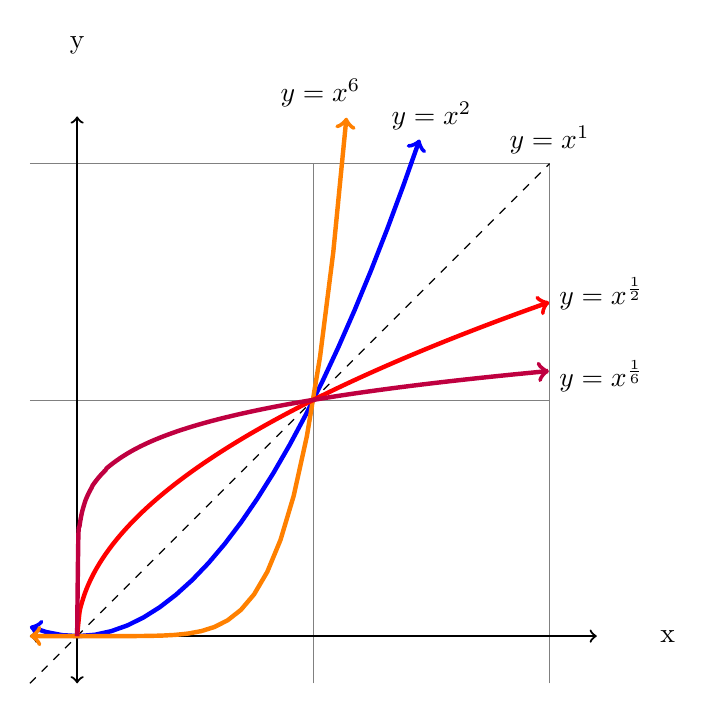
\begin{tikzpicture}[scale=3]
	\draw [help lines] (-0.2, -0.2) grid (2, 2);
	\draw [thick,<->] (-.2, 0) -- (2.2, 0);
	\draw [thick,<->] (0, -.2) -- (0, 2.2);
        % x-axis label
        \node at (2.5, 0) {x};
        % y-axis label
        \node at (0, 2.5) {y};

        \draw[dashed, -] (-.2,-.2) -- (2,2) node [anchor=south] {$y=x^1$};

        \draw[domain=-.2:1.45,<->,ultra thick,blue] plot (\x,\x*\x);
	\node at (1.5,2.1) [anchor=south] {$y=x^2$};

        \draw[domain=-.2:1.14,<->,ultra thick,orange] plot (\x,\x*\x*\x*\x*\x*\x);
	\node at (1.03,2.2) [anchor=south] {$y=x^6$};

        \draw[domain=0:2,->,ultra thick,red,samples=200,smooth] plot (\x,{sqrt(\x)});
	\node at (2,1.45) [anchor=west] {$y=x^{\frac{1}{2}}$};

        \draw[domain=0:2,->,ultra thick,purple,samples=400,smooth] plot (\x,{(\x)^(1/6)});
	\node at (2,1.1) [anchor=west] {$y=x^{\frac{1}{6}}$};
\end{tikzpicture}
\caption{Various power function graphs with exponents more and less than 1}
\end{centering}
\end{figure}

\subsection{Even, Odd, and Negative}
If the functions we are graphing are all of the type $f(x)=x^\frac{m}{n}$, then there will be
obvious patterns dependent upon what kind of numbers $m$ and $n$ are.  

\subsubsection{$n$ is odd}
If the root we are taken is odd, then it is easily defined for both positive and negative real input,
so the function will exist across the entire real domain.  In other words, there will be both a
left and right half.

\subsubsection{$n$ is even}
If the root we are taken is even, then negative inputs will be undefined.  Notice that this leads to
the major exception to our rule mentioned previously, that rational exponents are strictly equivalent
to powers over roots.  $\sqrt[4]{x^2}$ will work for negative inputs, but $x^\frac{1}{2}$ will not.

\subsubsection{$\frac{m}{n}$ is negative}
When an exponent is negative, that is equivalent to a positive exponent in the denominator.
These reciprocal transformations were covered in chapter 4.

\newpage
\subsection{Exercises}
\noindent\makebox[\textwidth]{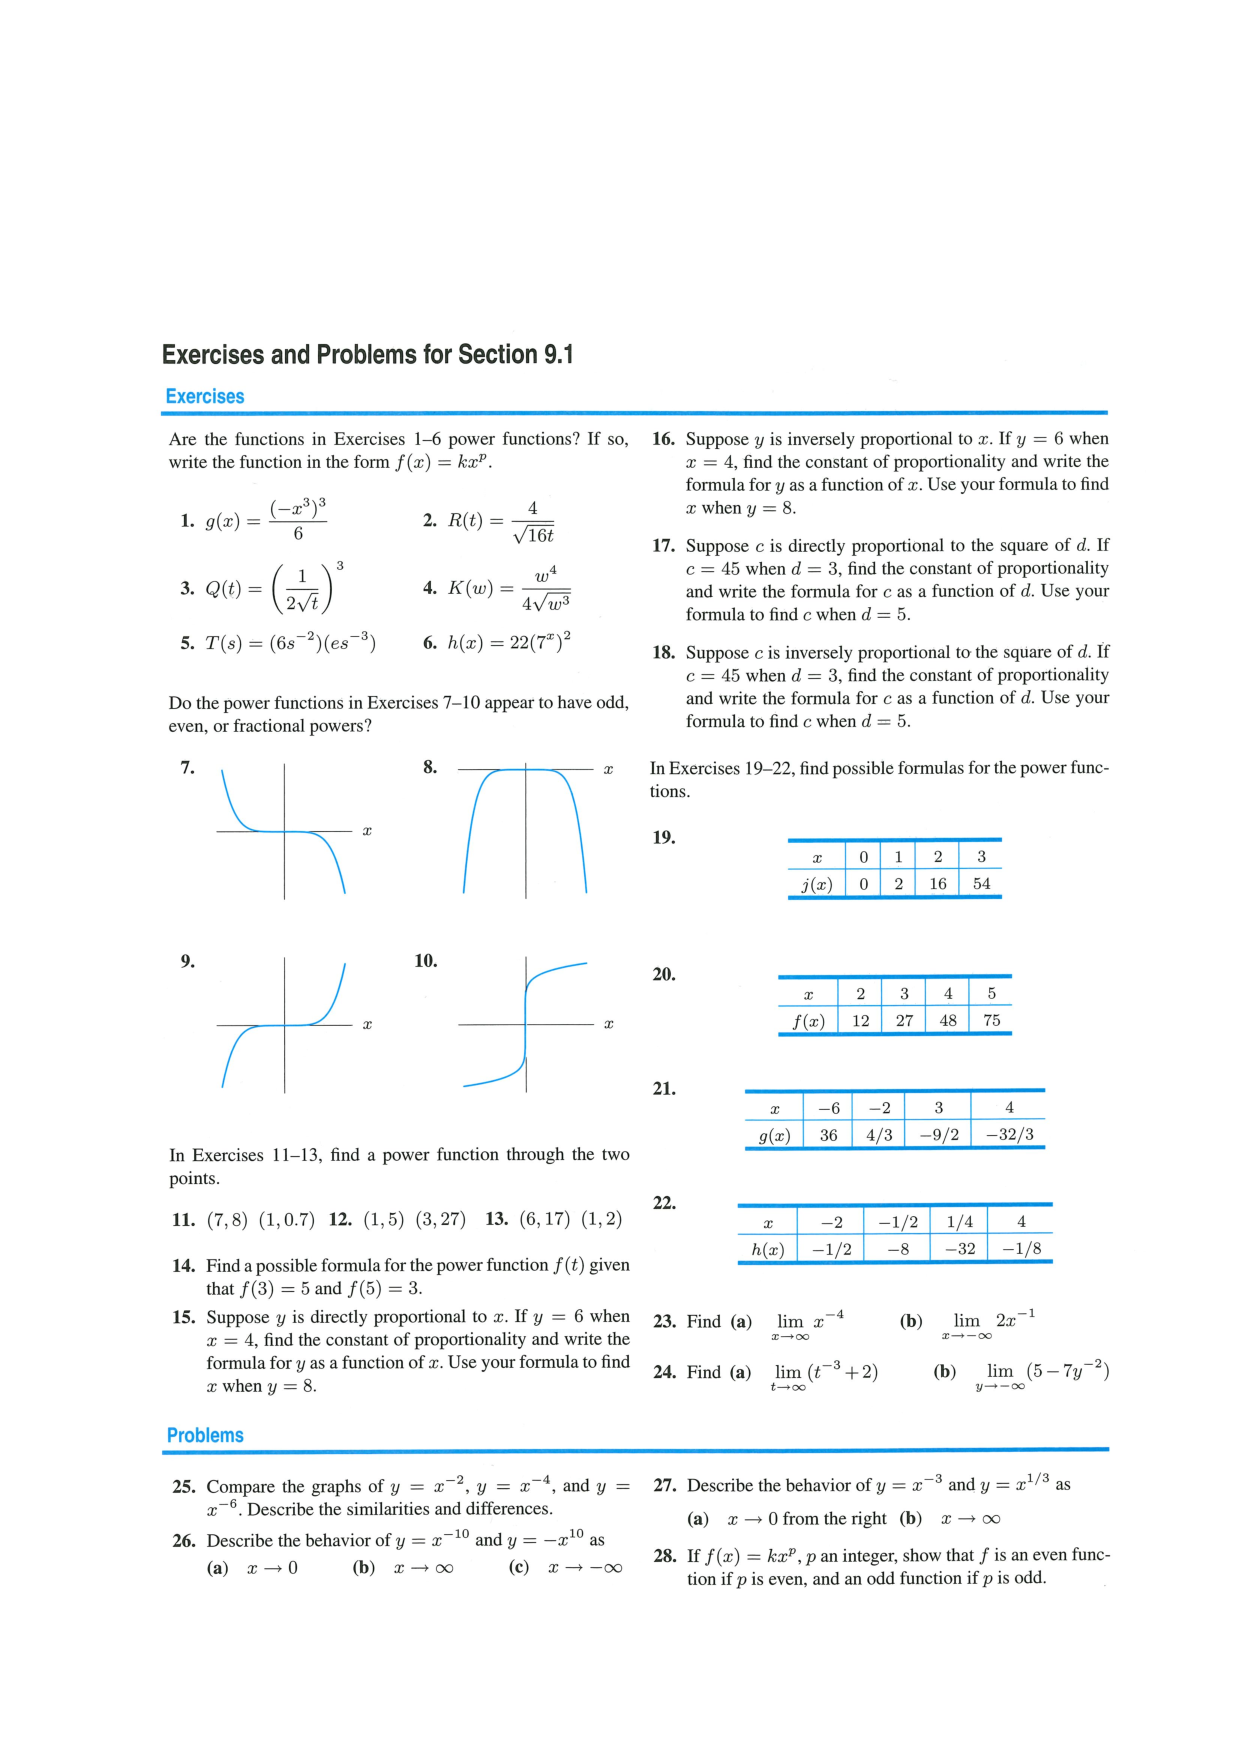
\includegraphics[width=\paperwidth]{\chapdir/0503xA.pdf}}
\newpage
\noindent\makebox[\textwidth]{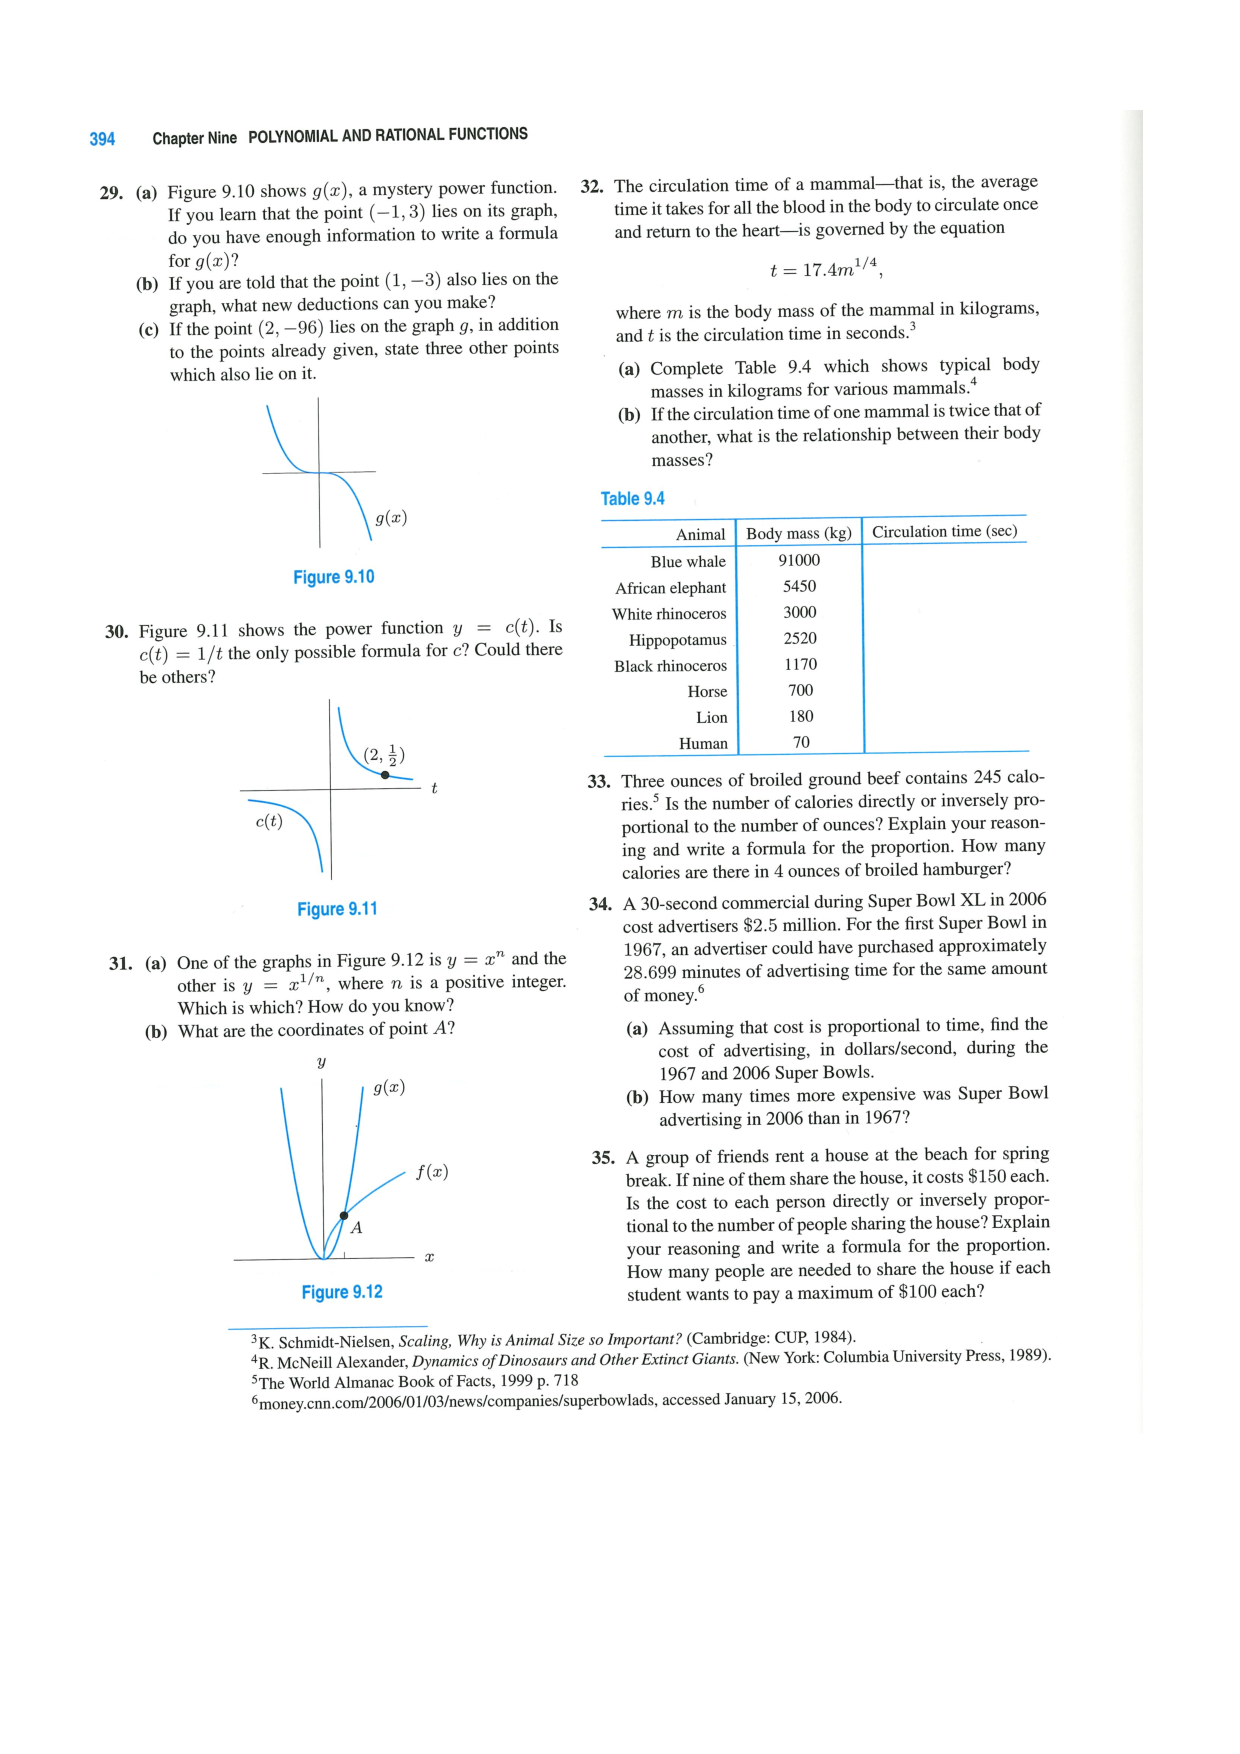
\includegraphics[width=\paperwidth]{\chapdir/0503xB.pdf}}
\newpage
\noindent\makebox[\textwidth]{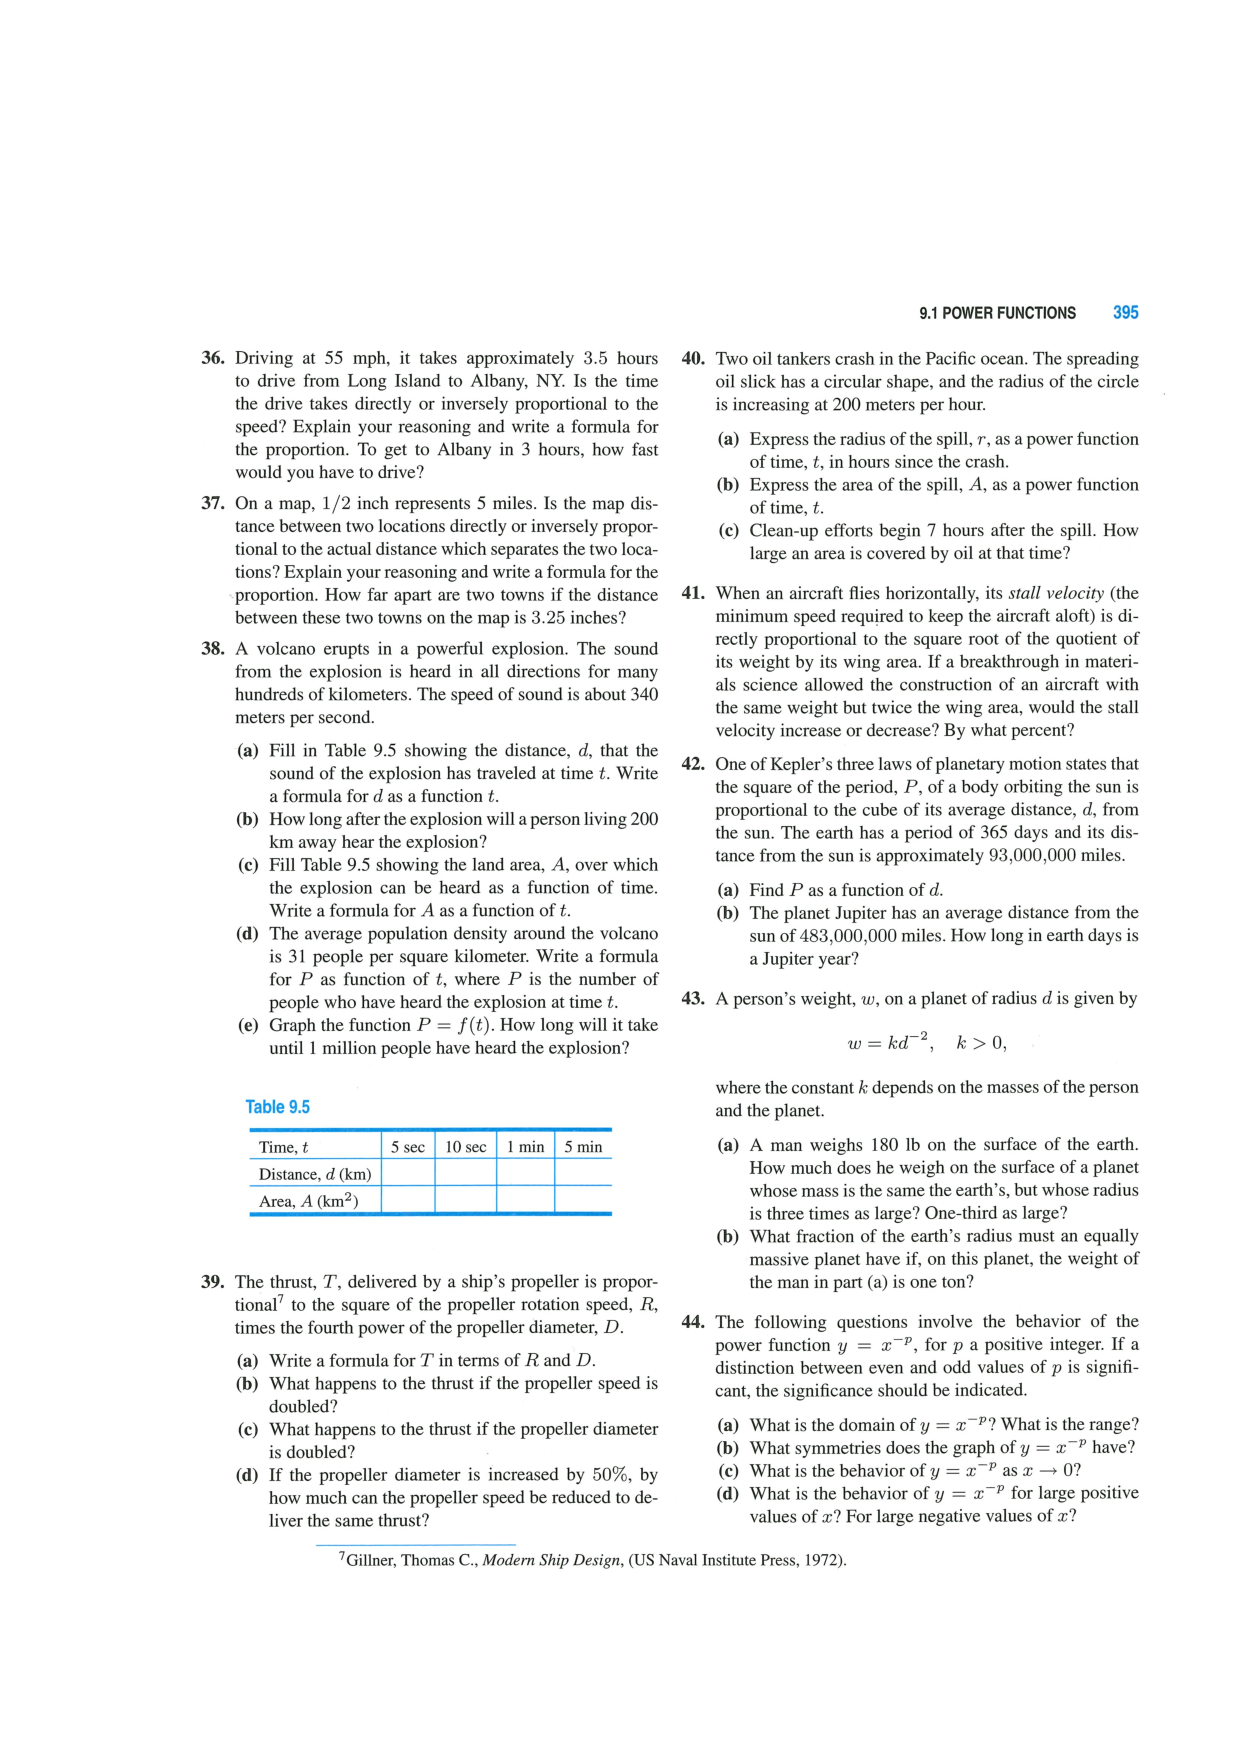
\includegraphics[width=\paperwidth]{\chapdir/0503xC.pdf}}
\newpage
\noindent\makebox[\textwidth]{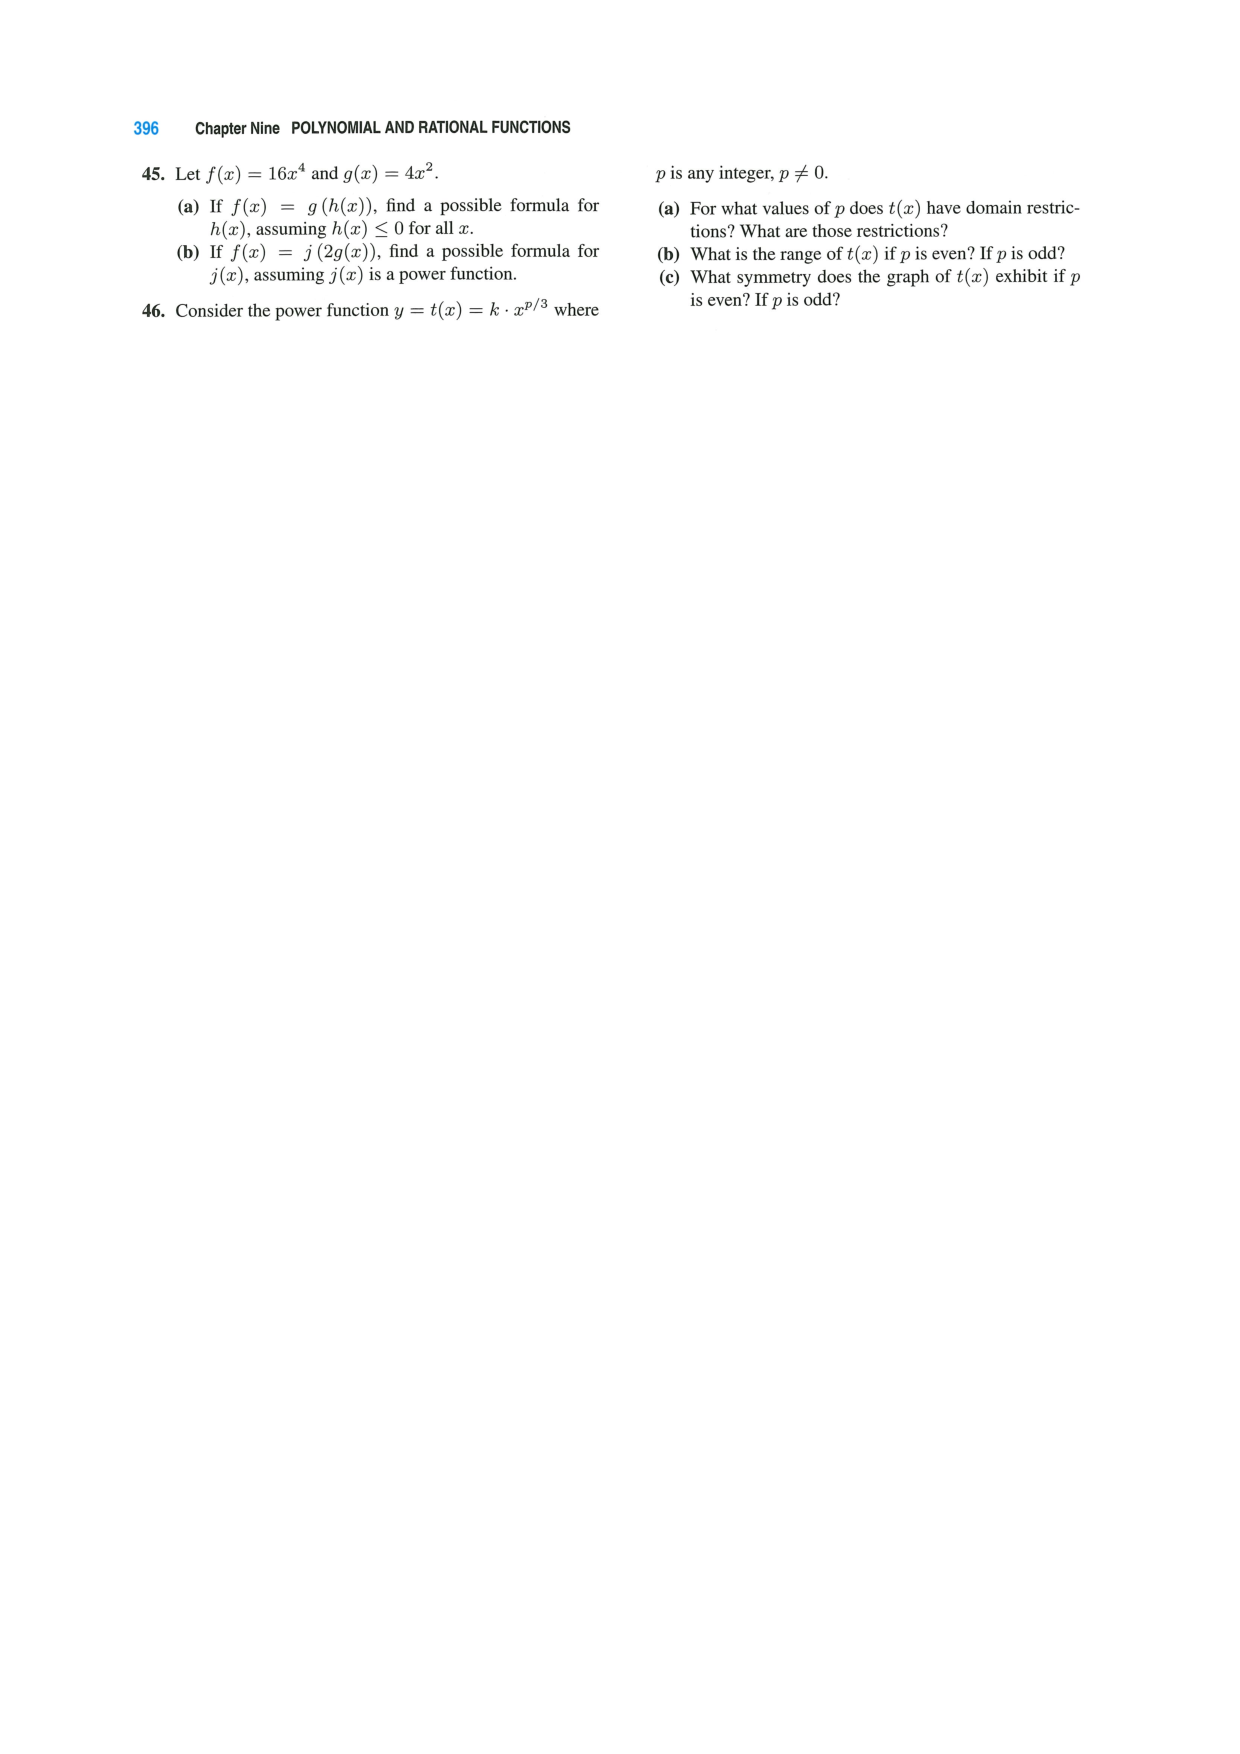
\includegraphics[width=\paperwidth]{\chapdir/0503xD.pdf}}



%									5 - 4
\newpage
\section{Concavity}
\subsection{Truth to Power}
in word
\newpage
%!TEX root =  ../main.tex

\objective{Find higher derivatives of functions, apply and produce their graphs}


\index{Concavity}
The first derivative of a function tell you the slope of the graph at any point.  When the
derivative function is positive, the original graph slopes up.  When it is negative the original
graph slopes down.  When it is zero, the original graph is flat.  

Could you graph the original function if you were given the derivative?  Well, you wouldn't 
know where to start, but once you picked a beginning, your slope would make it clear
where to go from there.  Practice staying within the graphical realm, drawing the derivative
of a given function, or a possible function given its derivative graph.


\subsection{Second Derivatives}
But what about the derivative of the derivative?
The slope of the slope is the rate of change, or acceleration.  Think about what happens when
you accelerate, even if you are traveling backwards at first: your velocity becomes more and more
positive.  On the other hand, deceleration means slowing down and quickly traveling backwards more and
more quickly.

\begin{figure}
\begin{centering}
\begin{tabular}{ |c|c|l| }
\hline
$f'(x)$ & $f''(x)$ & $f(x)$ \\ \hline \hline
\multirow{3}{*}{ + } & + & right side of a valley \\ \cline{2-3}
 & 0 & top of a peak \\ \cline{2-3}
 & - & left side of a mountain \\ \hline
\multirow{3}{*}{ 0 } & + & end of a valley, start of a peak \\ \cline{2-3}
 & 0 & plateau \\ \cline{2-3}
 & - & end of a peak, start of a valley \\ \hline
\multirow{3}{*}{ - } & + & ride side of a valley \\ \cline{2-3}
 & 0 & bottom of a valley \\ \cline{2-3}
 & - & right side of a peak \\
\hline
\end{tabular}
\caption{Relating first and second derivative signs to a graph}
\end{centering}
\end{figure}


Most of these behaviors can be seen in figure ...  The solid curve is $f(x)=\frac{1}{6}x^6
-2x^4+8x^2-20$.  The dashed curve is $f'(x)$ and the dotted is $f''(x)$.

\begin{figure}\label{derivativesigns}
\begin{centering}
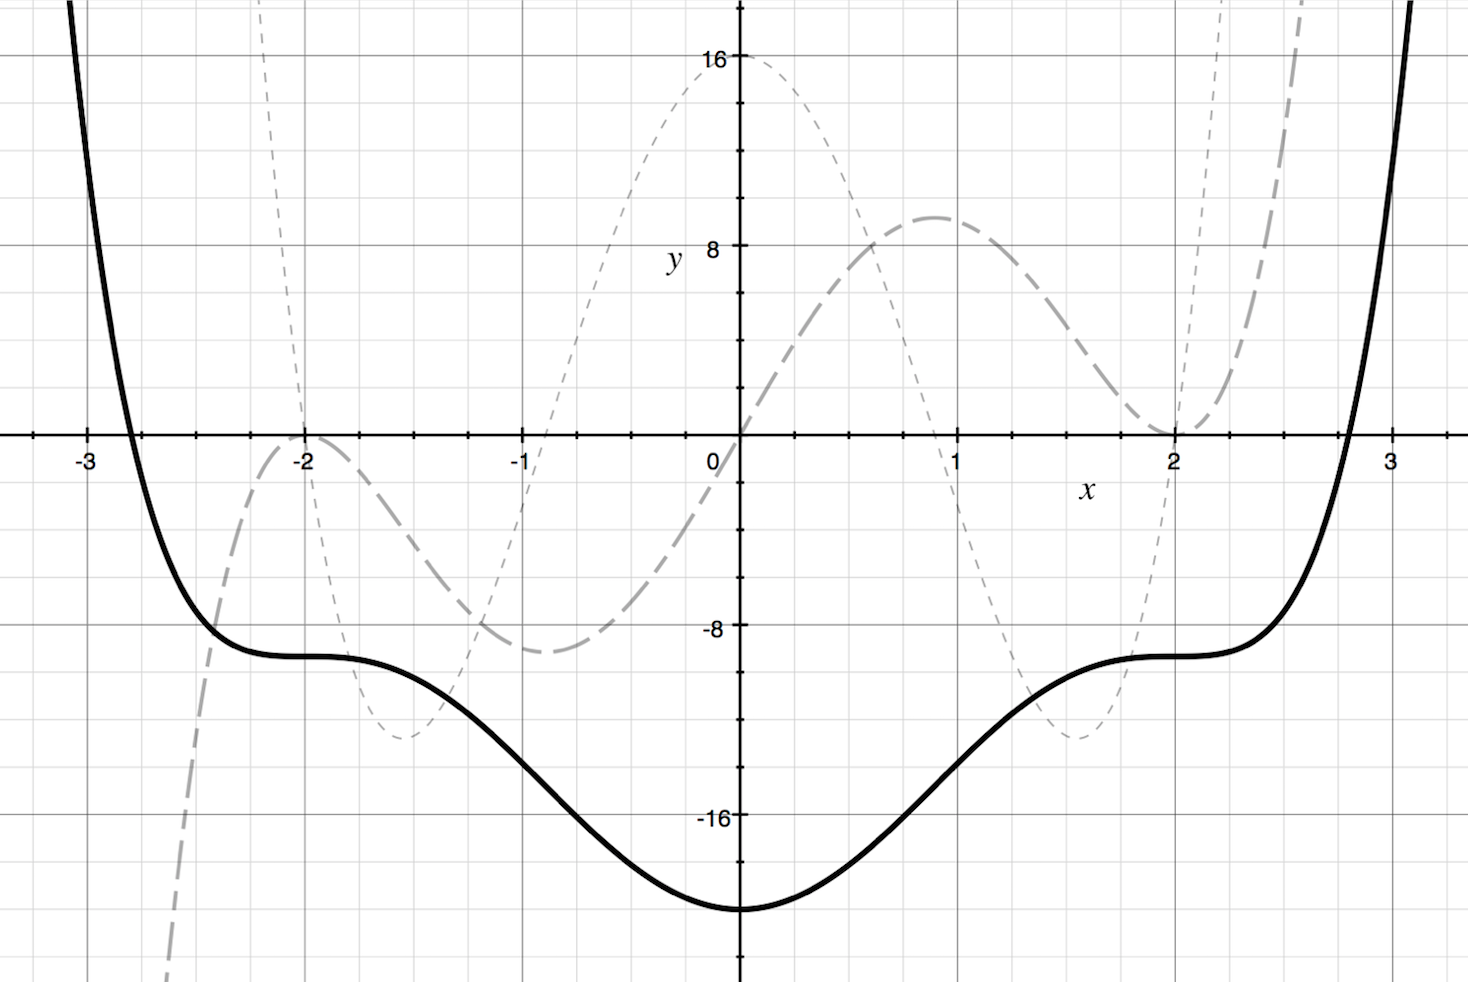
\includegraphics[width=\textwidth]{derivativesigns}
\caption{A function with inflection and turning points}
\end{centering}
\end{figure}


\newpage
\subsection{Exercises}
\noindent\makebox[\textwidth]{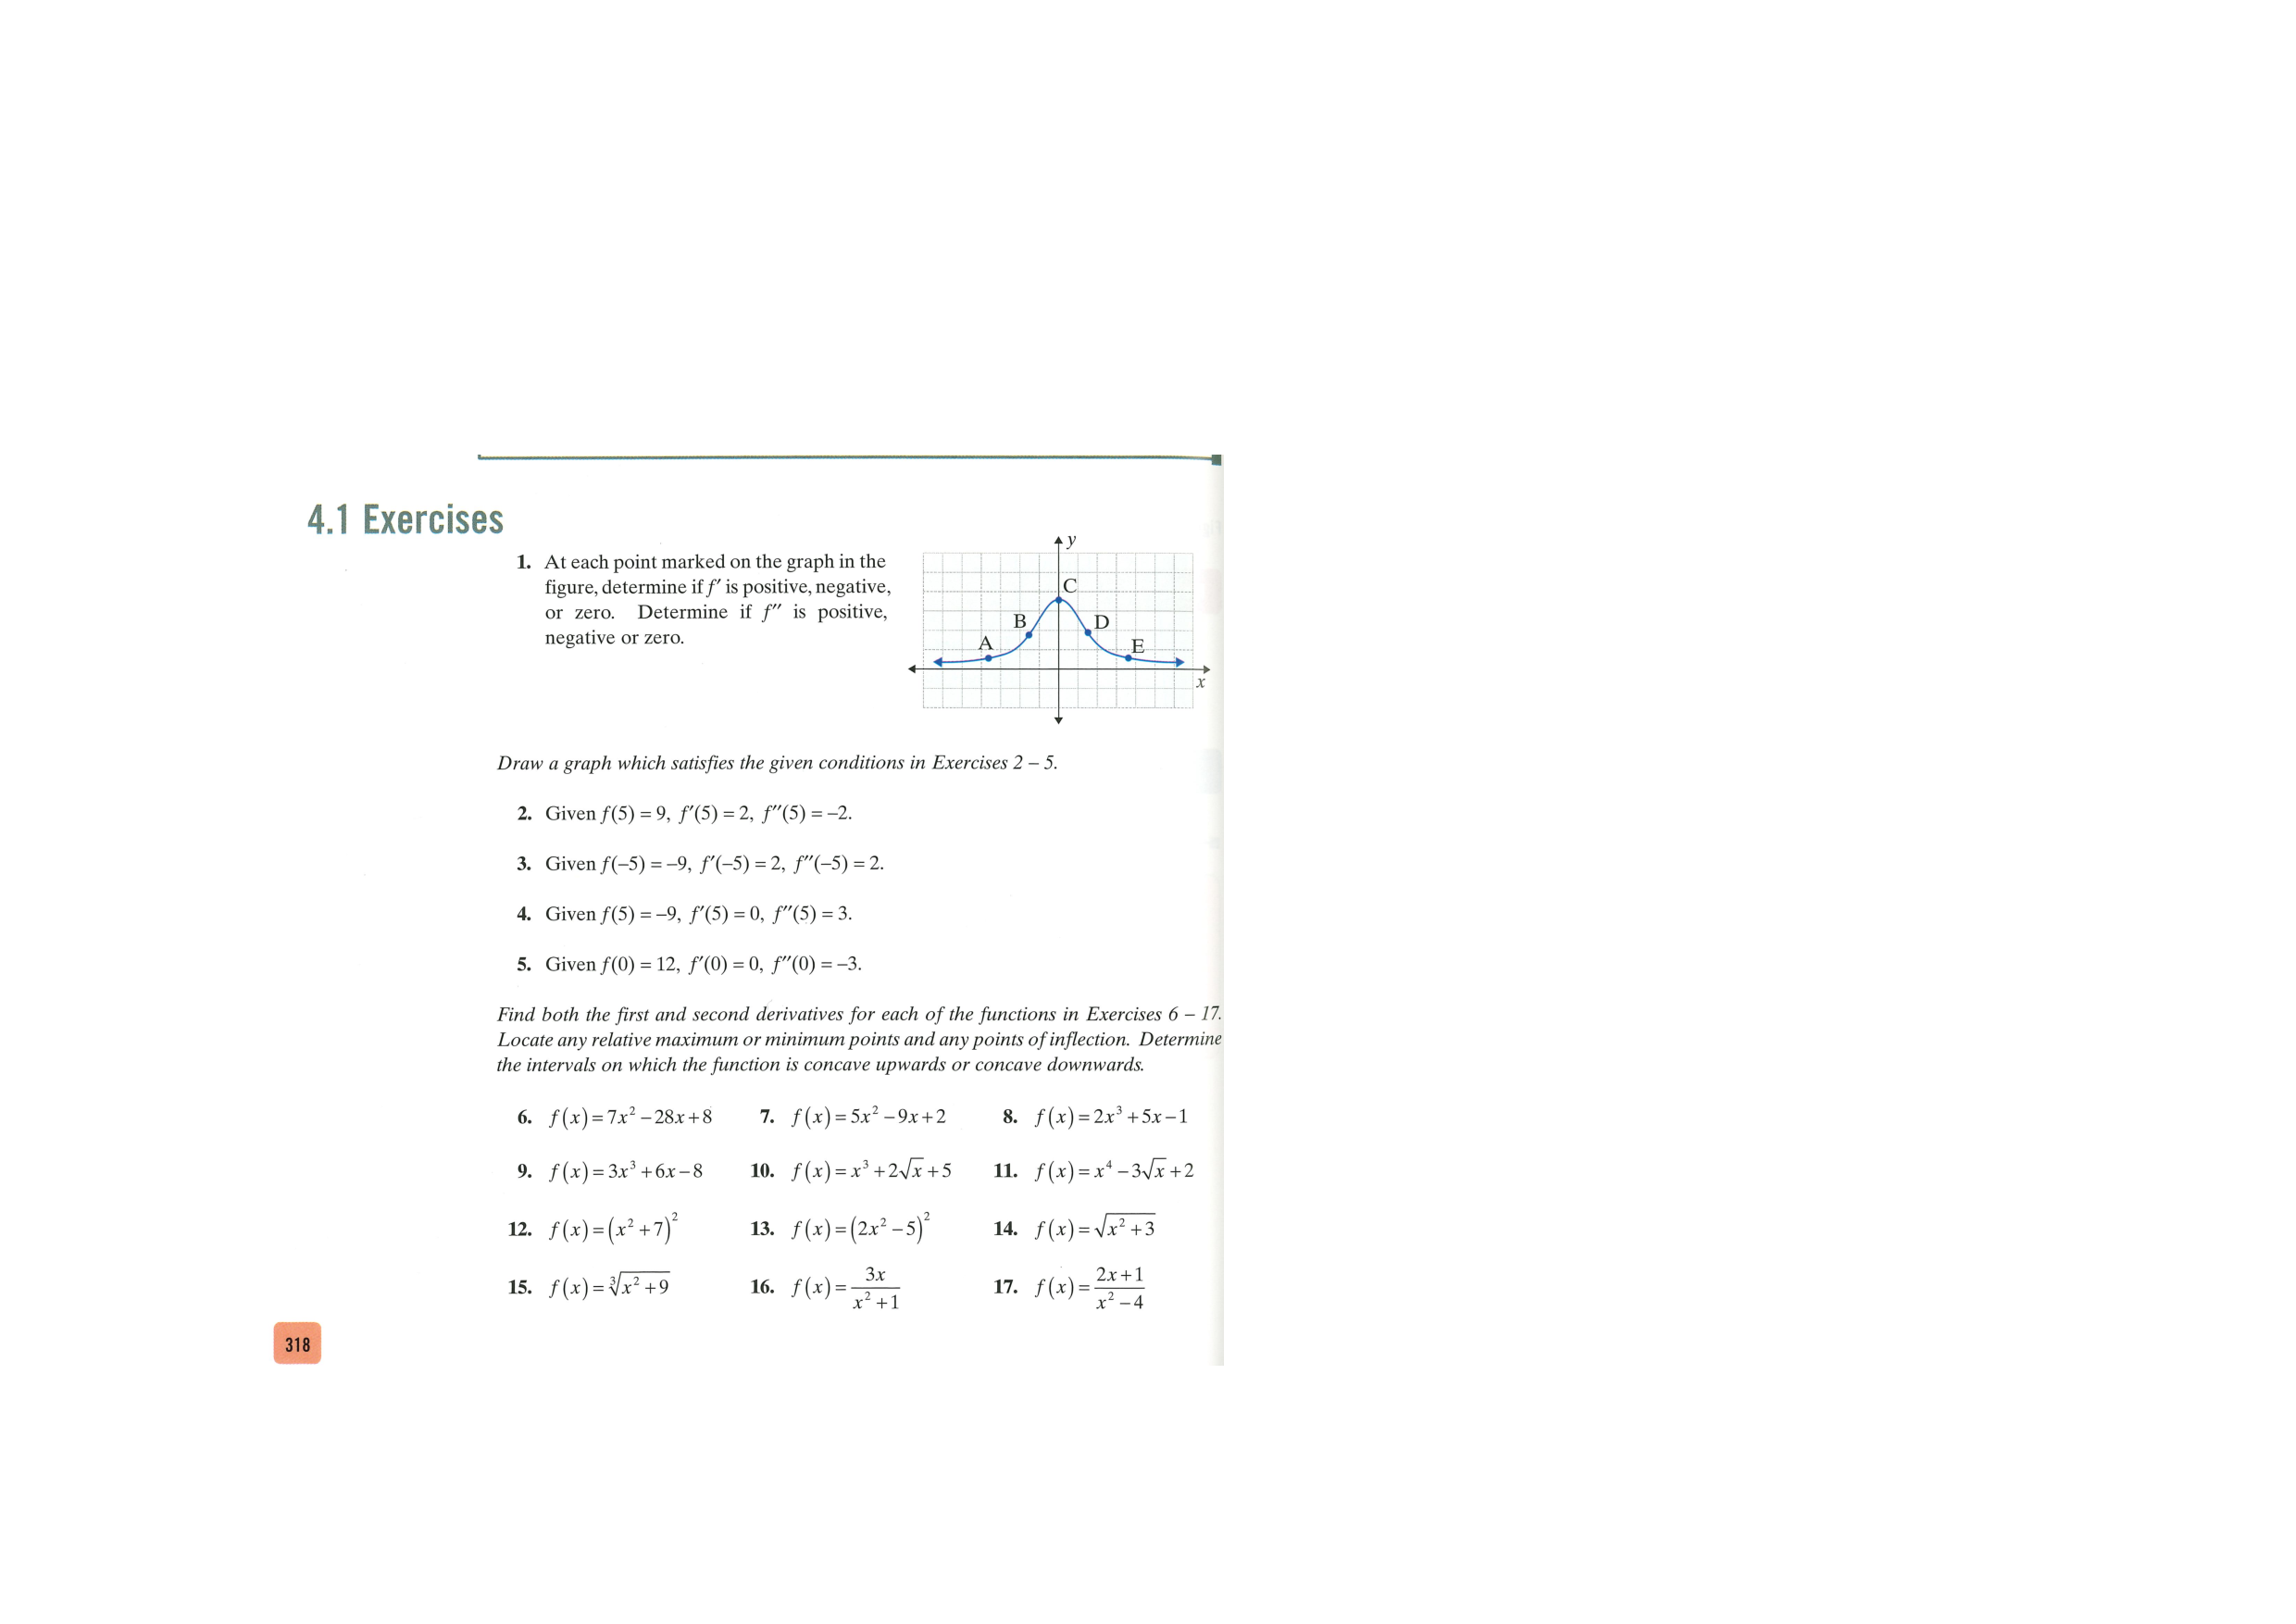
\includegraphics[width=\paperwidth]{\chapdir/0504xA.pdf}}
\newpage
\noindent\makebox[\textwidth]{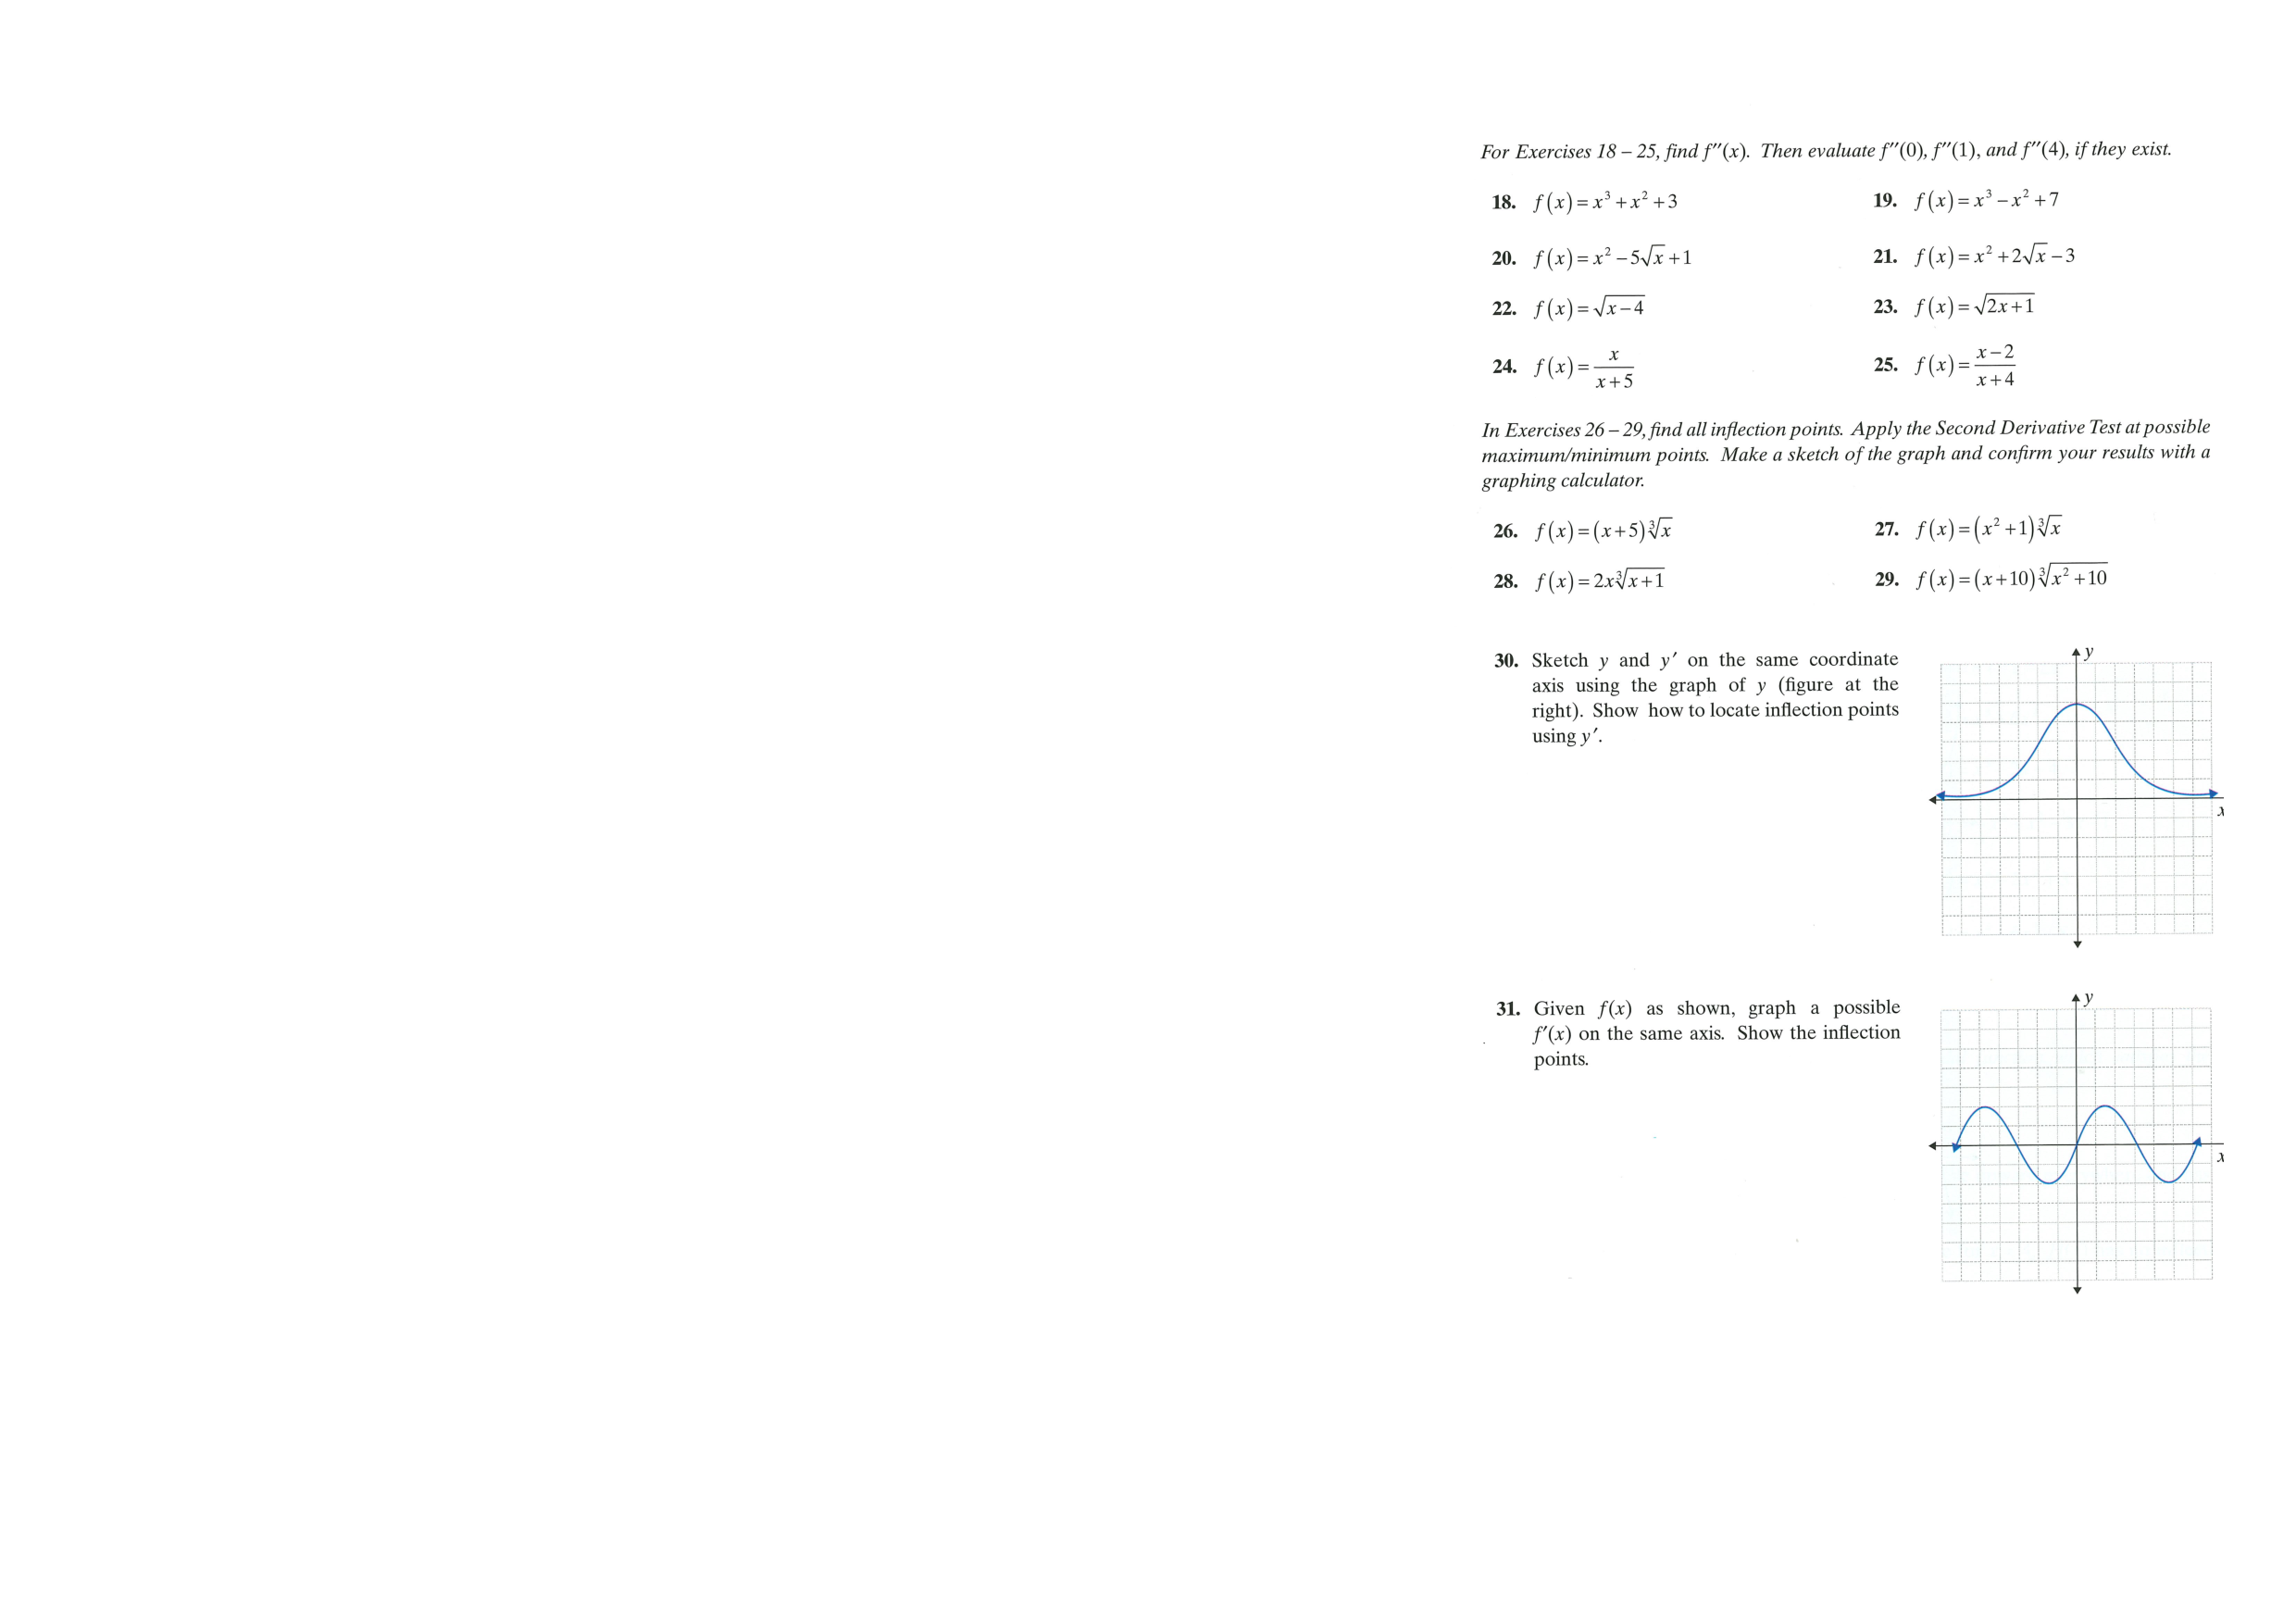
\includegraphics[width=\paperwidth]{\chapdir/0504xB.pdf}}
\newpage
\noindent\makebox[\textwidth]{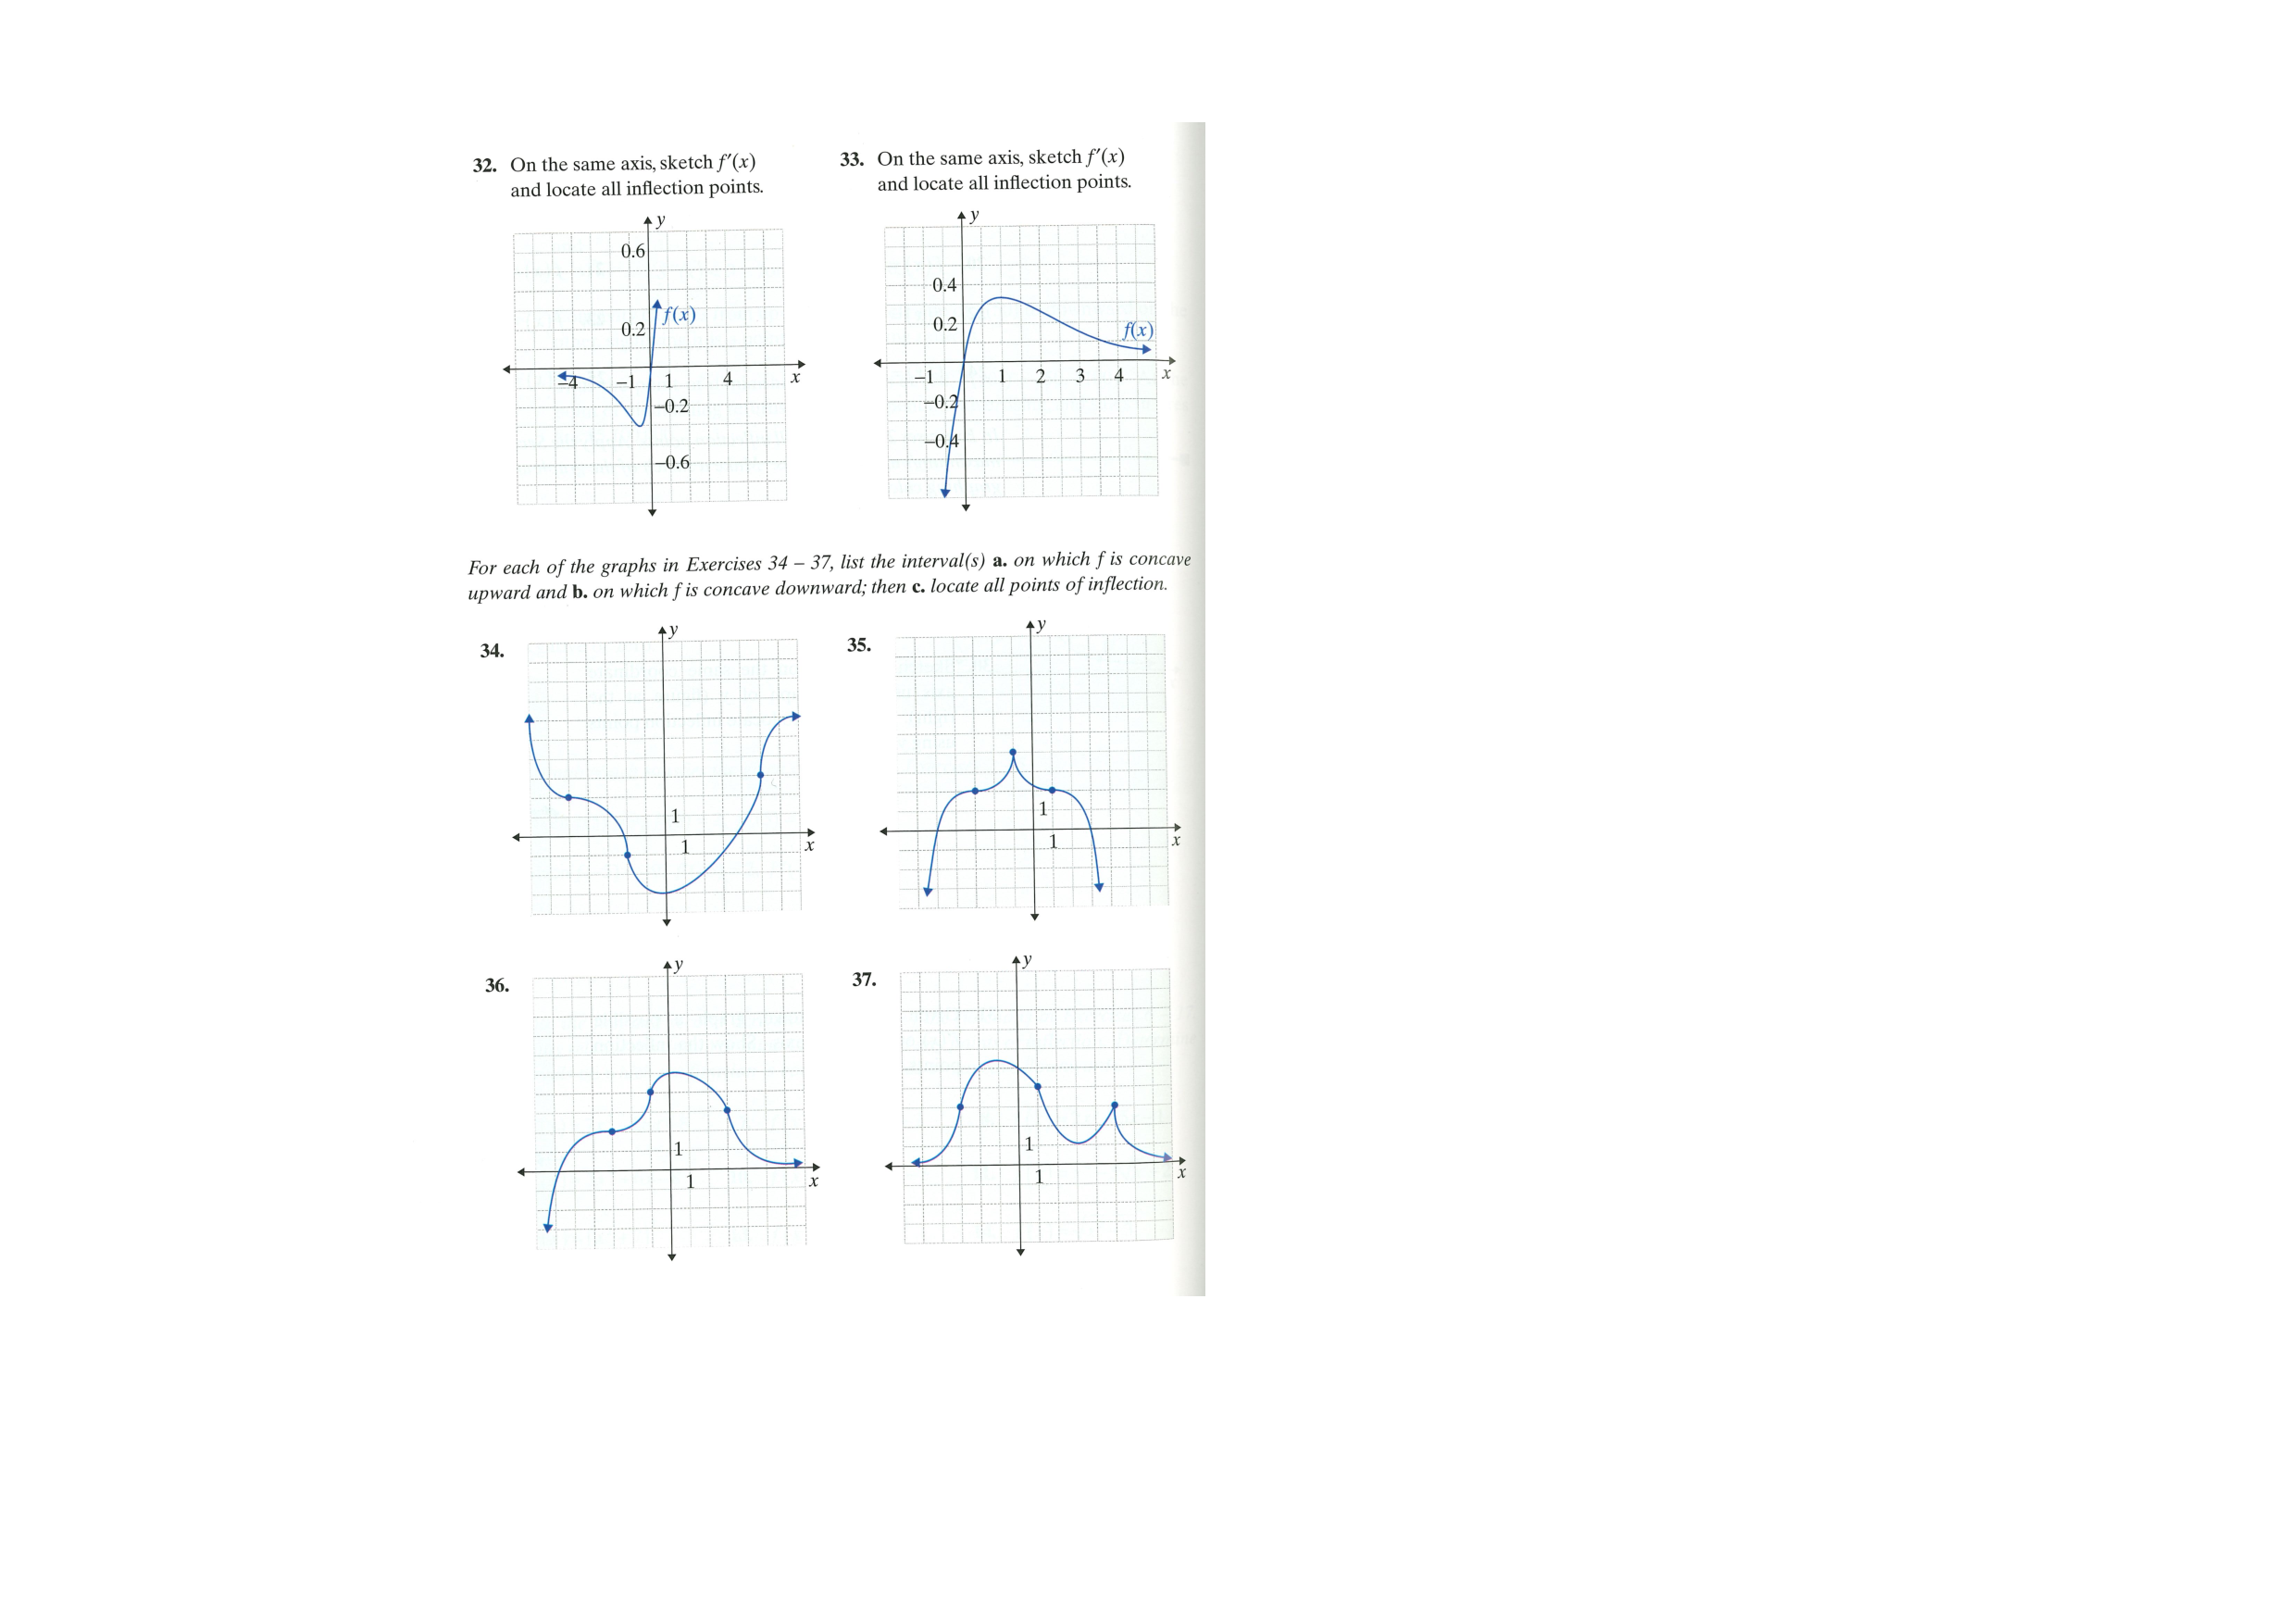
\includegraphics[width=\paperwidth]{\chapdir/0504xC.pdf}}
\newpage
\noindent\makebox[\textwidth]{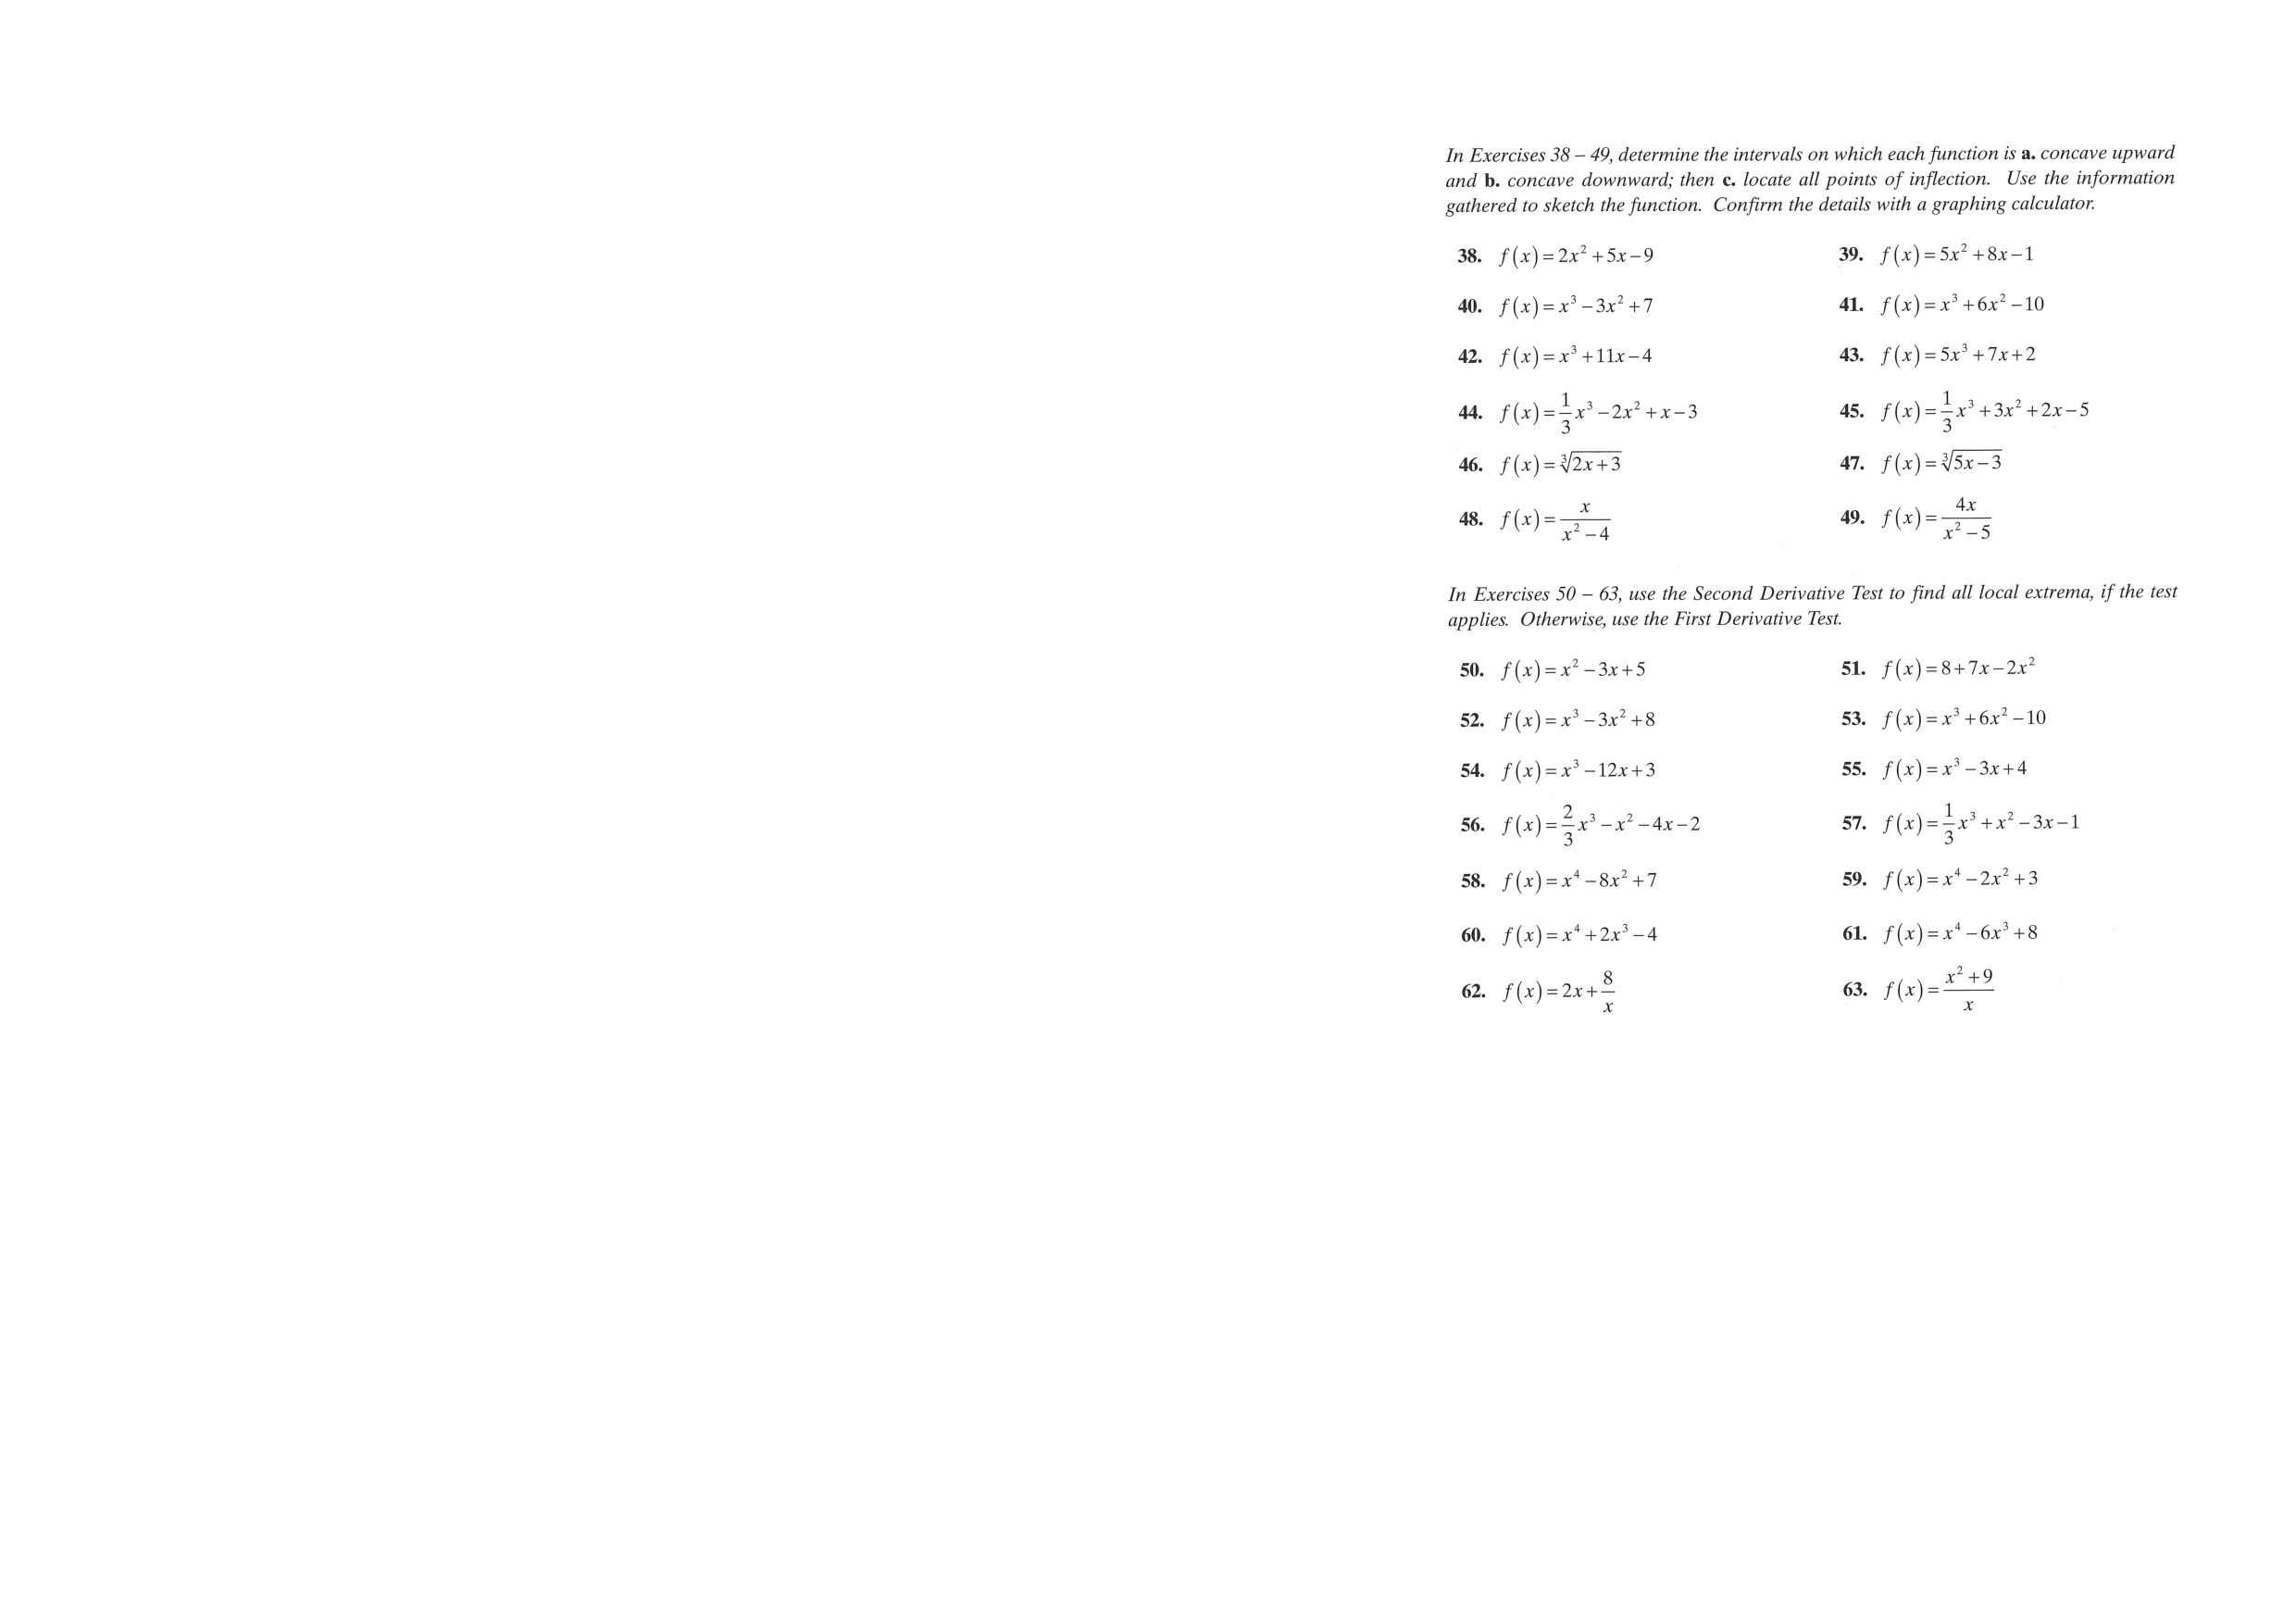
\includegraphics[width=\paperwidth]{\chapdir/0504xD.pdf}}
\newpage
\noindent\makebox[\textwidth]{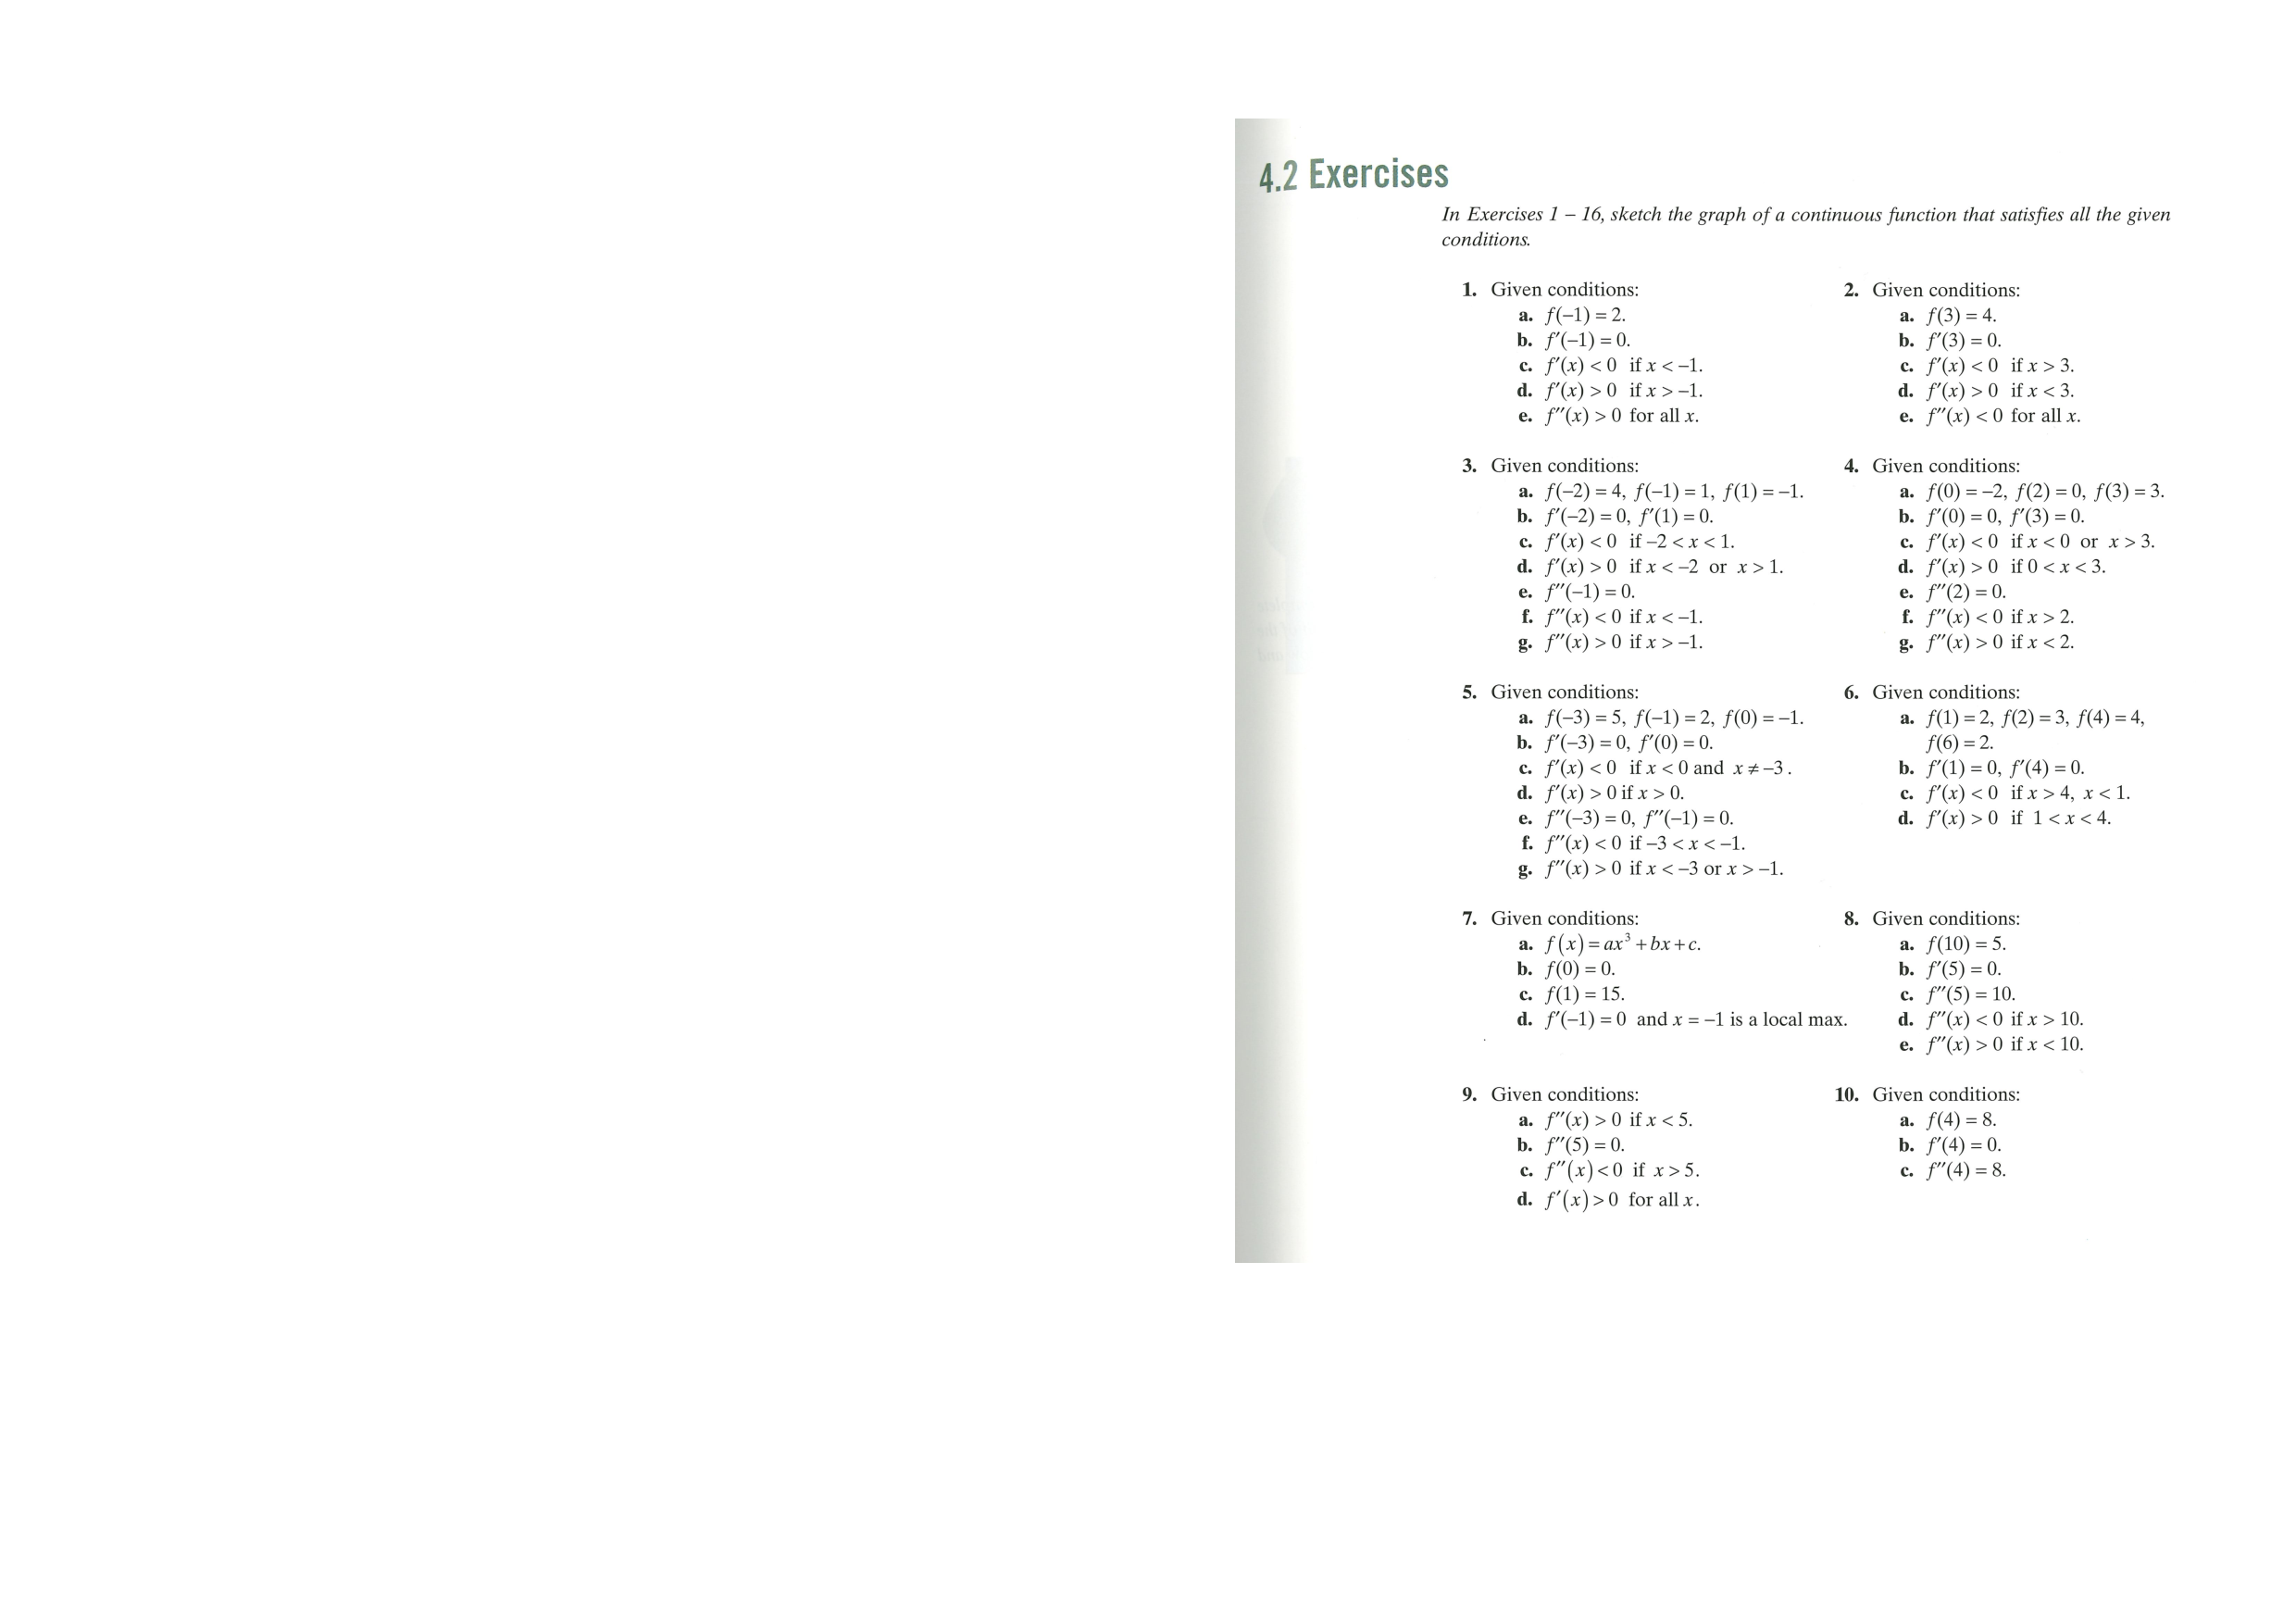
\includegraphics[width=\paperwidth]{\chapdir/0504xE.pdf}}


%									5 - 5
%\newpage
\invisiblesection{Integrals}
\subsection{Power in Motion}
\noindent\makebox[\textwidth]{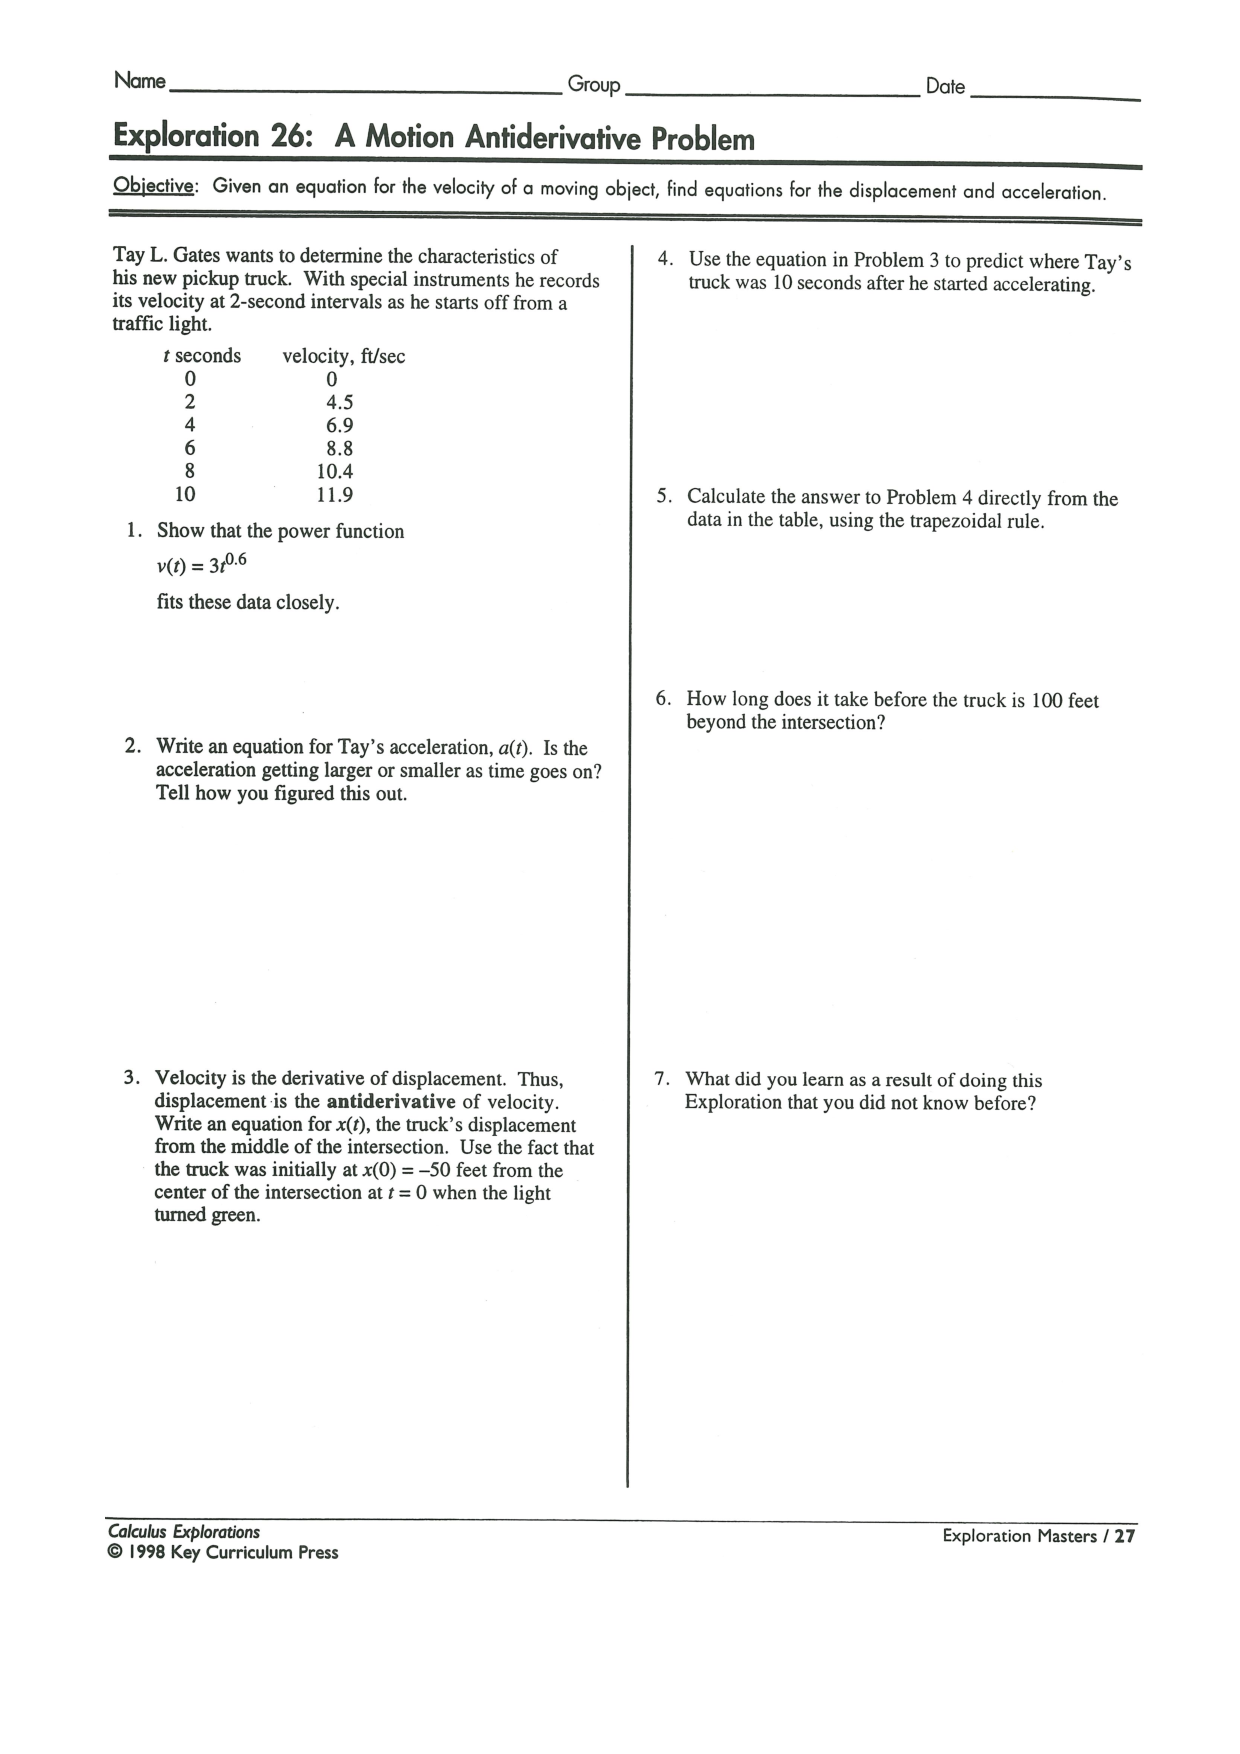
\includegraphics[width=\paperwidth]{\chapdir/0505p.pdf}}
%!TEX root =  ../main.tex

\subsection{Anti-Derivative}

\objective{Distinguish and find anti-derivatives and integrals of functions}


Suppose we are given a formula and are told it is the derivative of what we want.
This isn't as abstract as it sounds: velocity is the derivative of position, and (at least in 
many cars) it is easier to record velocity than it is position.  If the velocity
function is an algebraic equation, we simply need to apply the Power Rule
in reverse and we will have the anti-derivative of the equation.

The Power Rule states that the derivative of $x^n$ is $n\cdot x^{n-1}$.  In other words,
``take the exponent out front, and lower the exponent by one''.  If we wanted to
turn this backwards, in order to arrive at an exponent of $x^n$, we must have 
begun at $x^{n+1}$.  However, if we take the derivative of $x^{n+1}$, we must
multiply by $n+1$.  To cancel that, we should multiply by $\frac{1}{n+1}$.


\begin{derivation}{Backwards Power Rule}\index{Power Rule!Backwards}
The anti-derivative of $x^n$ is $\frac{1}{n+1} x^{n+1} + C$, where $C$ is an unknown
constant.
\end{derivation}


What is C?  Consider whether of not $x^2 +1$ is the anti-derivative of $\frac{1}{2}x$.
Is $x^2-1$?  Is $x^2+\pi$?  Because constants differentiate to 0, a constant could be 
part of our anti-derivative equation and we cannot know what it is, without more information.
What information?  Well, if we know the initial conditions (when $x=0$) then we can 
solve for $C$ and know precisely which anti-derivative equation we want.


\subsection{Integral}\index{integral!definite}
The preceding definition of anti-derivatives is very helpful algebraically, but what about
graphically?  If a given graph is the derivative of what we seek, can we interpret the
graph to give us numerical information?

Consider the graph of a car with constant velocity:

\begin{figure}[h]
\begin{centering}
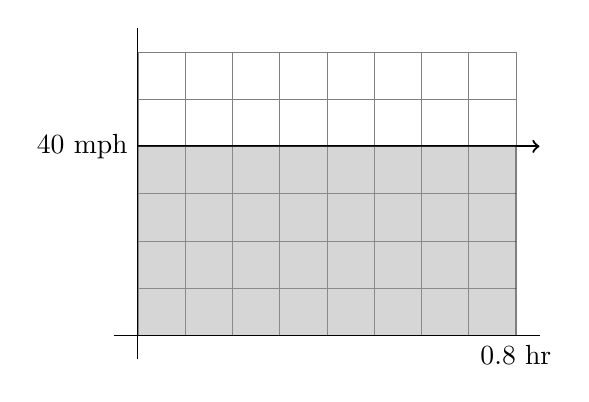
\begin{tikzpicture}[scale=0.6]
	\draw[help lines] (0,0) grid (8,6);
	\draw (-0.5,0) -- (8.5,0);
	\draw (0,-0.5) -- (0,6.5);
	\draw[thick,->] (0,4) node[anchor=east] {40 mph}-- (8.5,4);
	\draw (8,0) node[anchor=north] {0.8 hr};
	\draw [fill=gray!80,opacity =0.4] (0,0) rectangle (8,4);
\end{tikzpicture}
\caption{A car's velocity in 10's of mph, over tenths of an hour}
\end{centering}
\end{figure}


If we want position or distance, we have known a formula for a long time:
distance = rate $\cdot$ time.  The $y$-value is the rate.  The $x$-value is the 
time.  As hard as it may be to conceive of, distance is the \emph{area} under the
graph.  In this case, 40 mph times 0.8 hours is 32 miles.   Notice that this number does
not depend upon the initial position: the car has travelled 32 positive miles, regardless 
of where it began.

\begin{equation}
\int_0^{0.8}  40dx = \left.40x \right|_0^{0.8} = 40(.8) - 40(0) = 32
\end{equation}

What about more complicated velocity?  Let us begin with constant acceleration:

\begin{figure}[h]
\begin{centering}
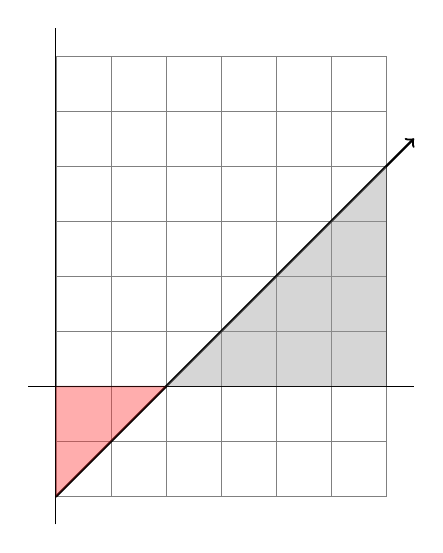
\begin{tikzpicture}[scale=0.7]
	\draw[help lines] (0,-2) grid (6,6);
	\draw (-0.5,0) -- (6.5,0);
	\draw (0,-2.5) -- (0,6.5);
	\draw [thick,->] (0,-2) -- (6.5,4.5);
	\draw [fill=red!80,opacity=0.4] (0,-2) -- (2,0) -- (0,0);
	\draw [fill=gray!80,opacity=0.4] (2,0) -- (6,0) -- (6,4);
\end{tikzpicture}
\caption{A car beginning at -20 mph but steadily accelerating to 40 mph by 0.6 hours later}
\end{centering}
\end{figure}

The object begins with a negative velocity, so we must count that distance as negative.
-2 + 8 = 6, so the object has gained that many units in positive displacement from 0 to 6.

In some problems, we can simply count the squares below the graph and find the
definite integral.  In most cases, the graph will be curved and we will need to find an
anti-derivative equation and subtract the evaluation at the left from that of the right.

Finally, notice that we can integrate functions we cannot differentiate, at times.  It would
be impossible for a physical object to have a velocity graph like the \texttt{int()} function,
but it can still be meaningful to find the area under the graph.

\begin{example}{Bandwidth Rates}
\exProblem
Suppose an wifi hotspot charges start at 2.50 per hour when you begin, and the rate goes
up .50 every 20 minutes after that.  The rate is not incremented
continuously, but jumps every 1/5 hour.  Illustrate the cost of using the service for 0.9 hours
as a definite integral.

\exSolution
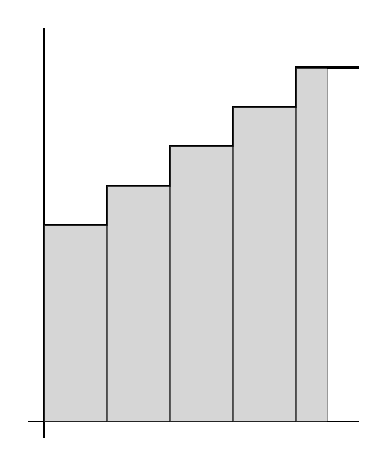
\begin{tikzpicture}[xscale=4,yscale=1]
	\draw (-0.05,0) -- (1,0) ;
	\draw (0,-.2) -- (0,5.0);
	\draw[thick] (0,2.50) -- (.2,2.5) -- (.2,3) -- (.4,3) -- (.4,3.5) -- (.6,3.5) -- (.6,4) -- (.8,4) -- (.8,4.5) -- (1,4.5);
	\draw [fill=gray!80,opacity=0.4] (0,0) rectangle (.2,2.5);
	\draw [fill=gray!80,opacity=0.4] (.2,0) rectangle (.4,3);
	\draw [fill=gray!80,opacity=0.4] (.4,0) rectangle (.6,3.5);
	\draw [fill=gray!80,opacity=0.4] (.6,0) rectangle (.8,4);
	\draw [fill=gray!80,opacity=0.4] (.8,0) rectangle (.9,4.5);
\end{tikzpicture}
As the rectangle illustrate, $(0.2)(2.5) + (0.2)(3.0) + (0.2)(3.5) + (0.2)(4.0) + (0.1)(4.5) = 3.05$.
\end{example}


~\vfill
\subsection{Exercises}
\noindent\makebox[\textwidth]{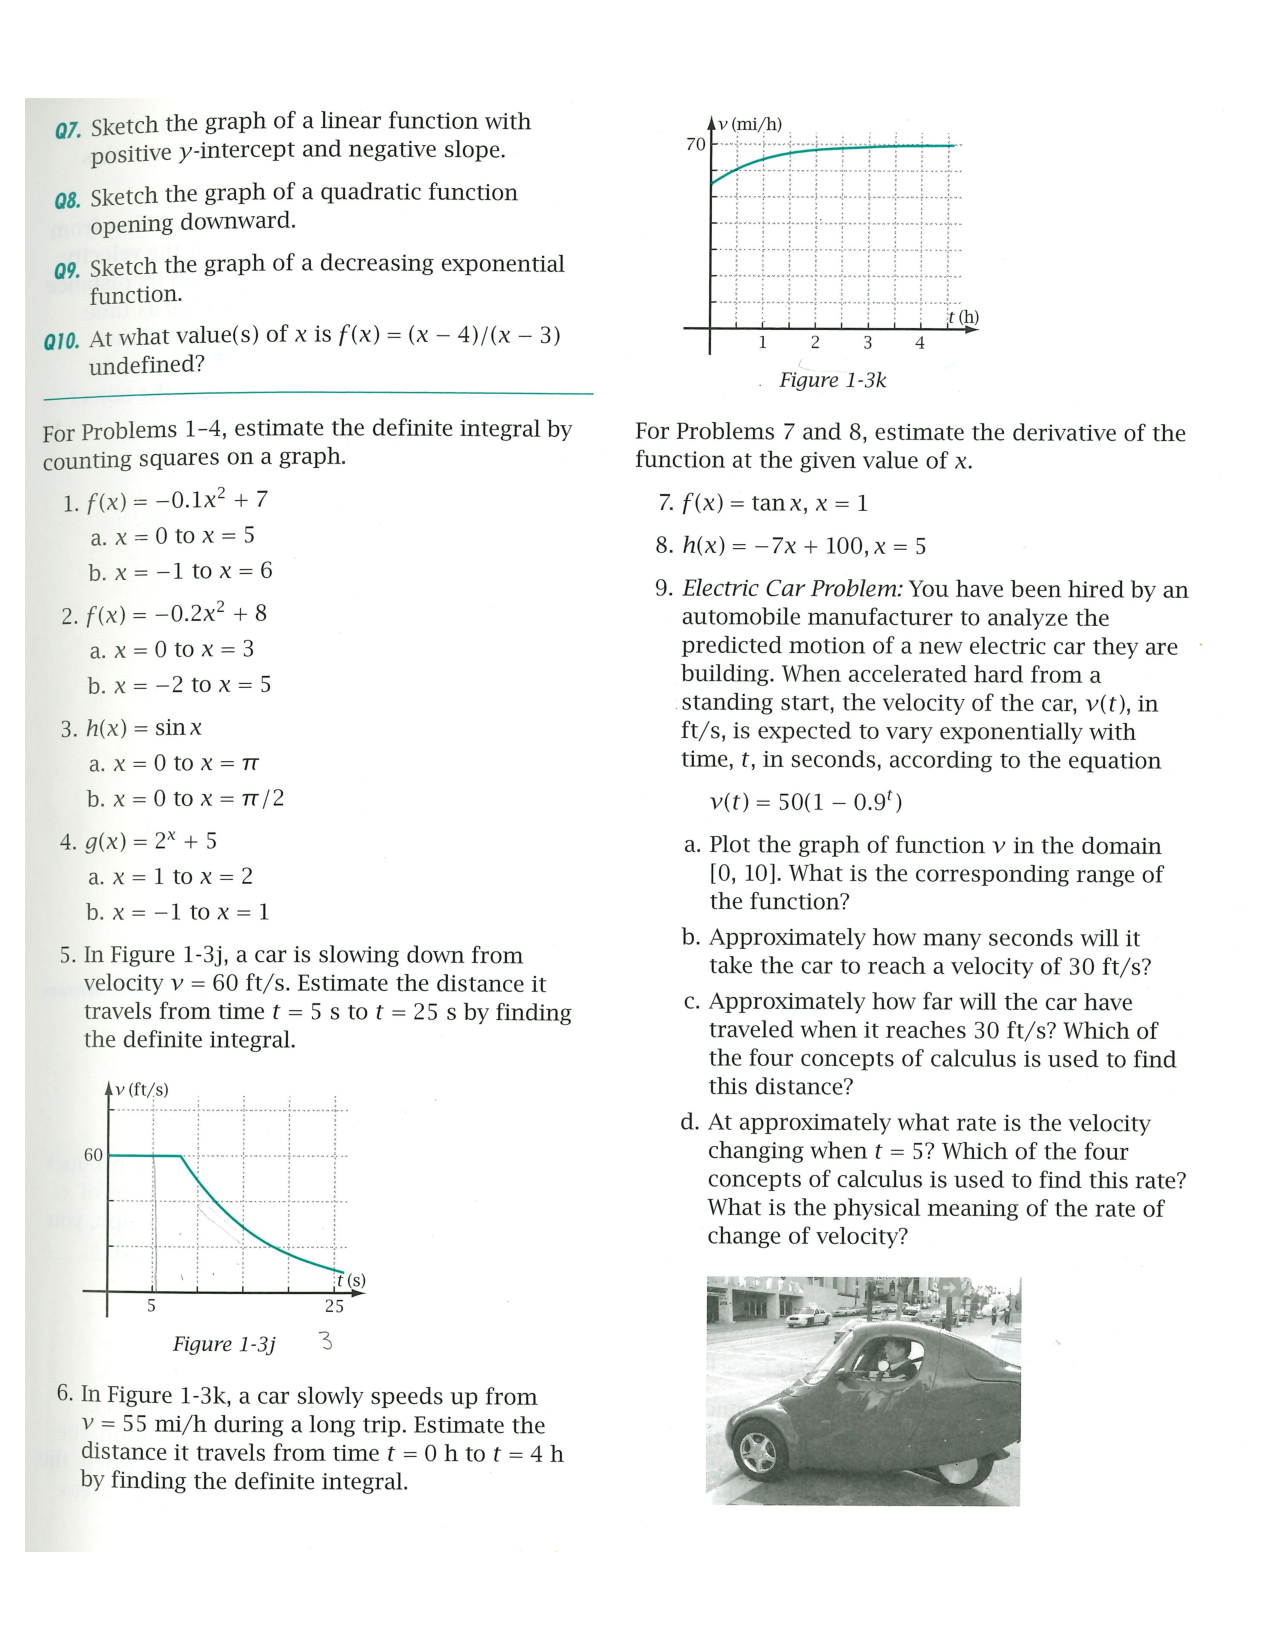
\includegraphics[width=\paperwidth]{\chapdir/0505xA.pdf}}
\newpage
\noindent\makebox[\textwidth]{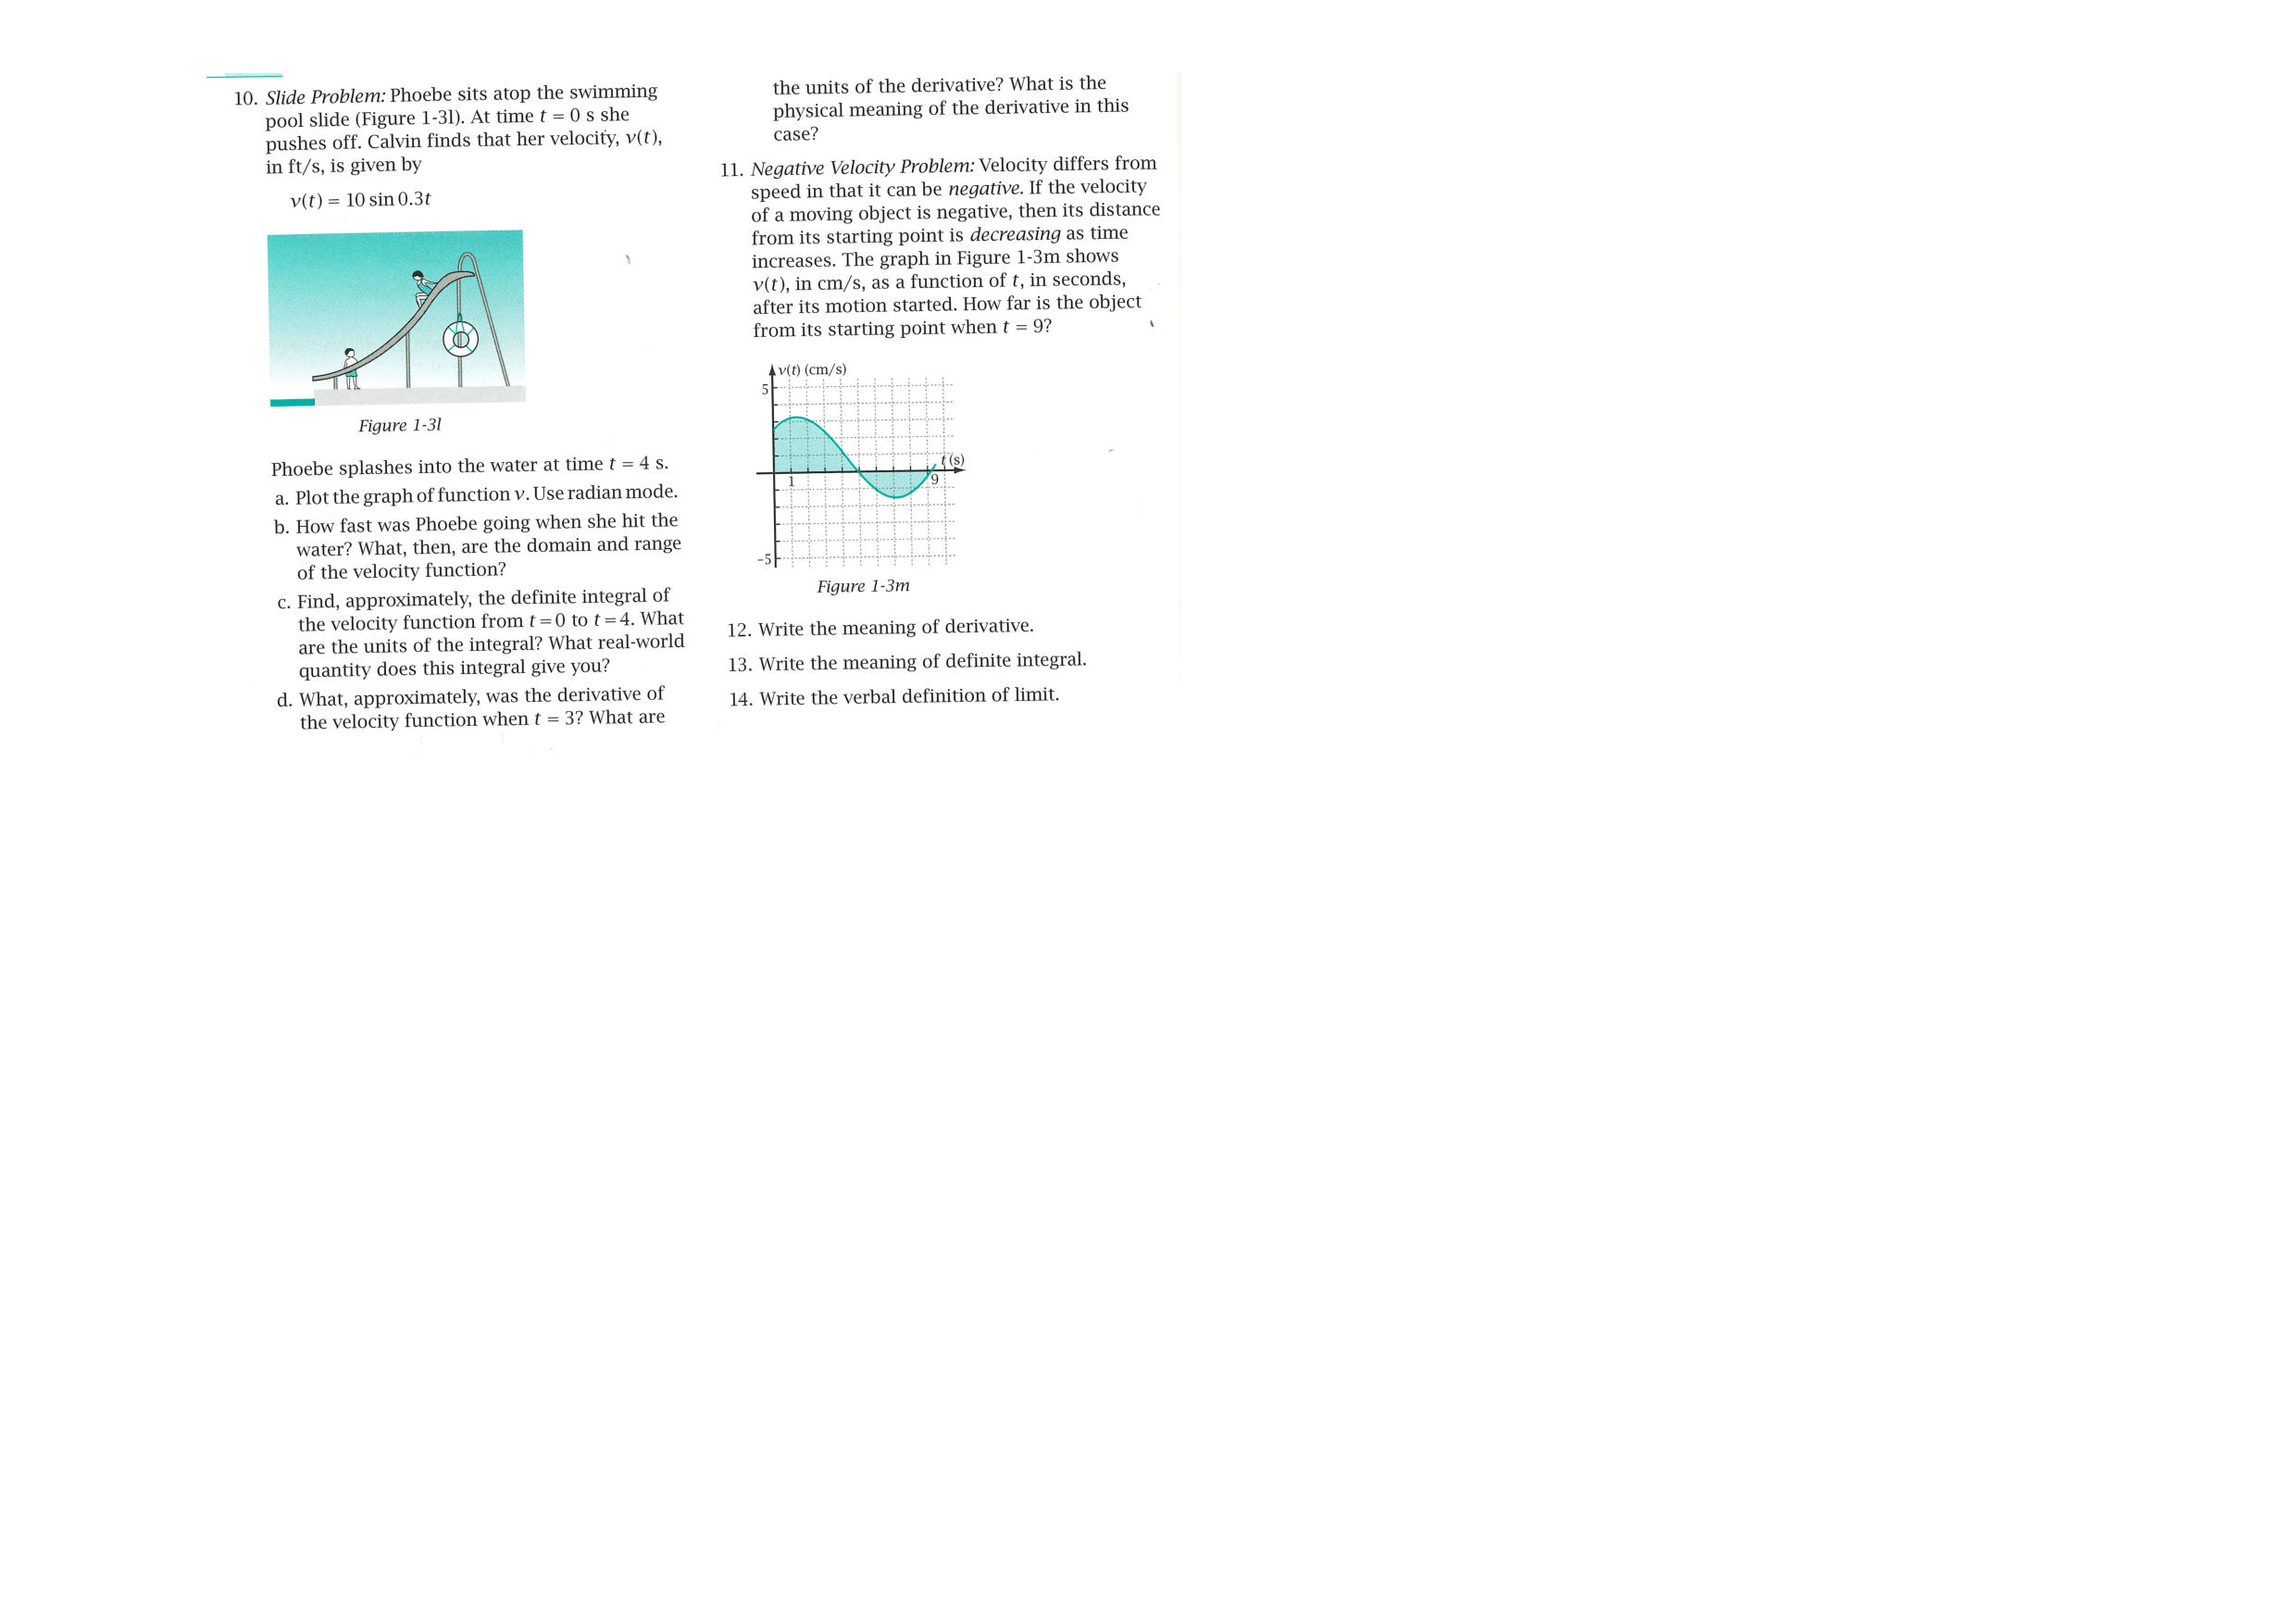
\includegraphics[width=\paperwidth]{\chapdir/0505xB.pdf}}



\newpage
\section{Review}
\subsection{Chapter Review}
\subsection{Chapter Test}